%%%%%%%%%%%%%%%%%%%%%%%%%%%%%%%%%%%%%%%%%%%%%%%%%%%%%%%%%%%%%%%%%%%%%%%%

%%% LaTeX Template for AAMAS-2025 (based on sample-sigconf.tex)
%%% Prepared by the AAMAS-2025 Program Chairs based on the version from AAMAS-2025. 

%%%%%%%%%%%%%%%%%%%%%%%%%%%%%%%%%%%%%%%%%%%%%%%%%%%%%%%%%%%%%%%%%%%%%%%%

%%% Start your document with the \documentclass command.


%%% == IMPORTANT ==
%%% Use the first variant below for the final paper (including auithor information).
%%% Use the second variant below to anonymize your submission (no authoir information shown).
%%% For further information on anonymity and double-blind reviewing, 
%%% please consult the call for paper information
%%% https://aamas2025.org/index.php/conference/calls/submission-instructions-main-technical-track/

%%%% For anonymized submission, use this
\documentclass[sigconf,anonymous]{aamas} 

%%%% For camera-ready, use this
%\documentclass[sigconf]{aamas} 
\newtheorem{remark}{Remark}

%%% Load required packages here (note that many are included already).

\usepackage{balance} % for balancing columns on the final page
\usepackage{macros}
\usepackage{mathrsfs}
\usepackage{tikz}
\usepackage{bussproofs}
\usepackage{algorithm}
\usepackage{algpseudocode}
\usetikzlibrary{shapes.misc, fit, decorations.pathreplacing,calligraphy,positioning} %for crossing-out arrows and rectangles around nodes

\usepackage{soul}
\usepackage{todonotes}
\newcommand\rustam[1]{\todo[color=blue!30,size=\small,inline]{Rustam: #1}}
\newcommand\davide[1]{\todo[color=green!30,size=\small,inline]{Davide: #1}}
\newcommand{\rev}[1]{{\color{blue} #1}}
 %\newcommand{\rev}[1]{{#1}}
 \newcommand{\rem}[1]{{\color{red} #1}}

 \algtext*{EndIf}
\algtext*{EndFor}
\renewcommand{\sl}{\mathfrak{sl}}

\algnewcommand\algorithmiccase{\textbf{case}}
\algdef{SE}[CASE]{Case}{EndCase}[1]{\algorithmiccase\ #1}{\algorithmicend\ \algorithmiccase}%
\algtext*{EndCase}

\makeatletter
\newenvironment{breakablealgorithm}
  {% \begin{breakablealgorithm}
   \begin{center}
     \refstepcounter{algorithm}% New algorithm
     \hrule height.8pt depth0pt \kern2pt% \@fs@pre for \@fs@ruled
     \renewcommand{\caption}[2][\relax]{% Make a new \caption
       {\raggedright\textbf{\fname@algorithm~\thealgorithm} ##2\par}%
       \ifx\relax##1\relax % #1 is \relax
         \addcontentsline{loa}{algorithm}{\protect\numberline{\thealgorithm}##2}%
       \else % #1 is not \relax
         \addcontentsline{loa}{algorithm}{\protect\numberline{\thealgorithm}##1}%
       \fi
       \kern2pt\hrule\kern2pt
     }
  }{% \end{breakablealgorithm}
     \kern2pt\hrule\relax% \@fs@post for \@fs@ruled
   \end{center}
  }
\makeatother



%%%%%%%%%%%%%%%%%%%%%%%%%%%%%%%%%%%%%%%%%%%%%%%%%%%%%%%%%%%%%%%%%%%%%%%%

%%% AAMAS-2025 copyright block (do not change!)

\setcopyright{ifaamas}
\acmConference[AAMAS '25]{Proc.\@ of the 24th International Conference
on Autonomous Agents and Multiagent Systems (AAMAS 2025)}{May 19 -- 23, 2025}
{Detroit, Michigan, USA}{A.~El~Fallah~Seghrouchni, Y.~Vorobeychik, S.~Das, A.~Nowe (eds.)}
\copyrightyear{2025}
\acmYear{2025}
\acmDOI{}
\acmPrice{}
\acmISBN{}


%%%%%%%%%%%%%%%%%%%%%%%%%%%%%%%%%%%%%%%%%%%%%%%%%%%%%%%%%%%%%%%%%%%%%%%%

%%% == IMPORTANT ==
%%% Use this command to specify your EasyChair submission number.
%%% In anonymous mode, it will be printed on the first page.

\acmSubmissionID{710}

%%% Use this command to specify the title of your paper.

\title[Coalition Strategy Logic]{Coalition Strategy Logic}

%%% Provide names, affiliations, and email addresses for all authors.

\author{Davide Catta}
\affiliation{
  \institution{Camelot Castle}
  \city{Camelot}
  \country{United Kingdom}}
\email{king.arthur@camelot.uk}

\author{Rustam Galimullin}
\affiliation{
  \institution{The Lady's Lake}
  \city{Avalon}
  \country{United Kingdom}}
\email{lady.of.the.lake@avalon.uk}

\author{Aniello Murano}
\affiliation{
  \institution{The Lady's Lake}
  \city{Avalon}
  \country{United Kingdom}}
\email{lady.of.the.lake@avalon.uk}

%%% Use this environment to specify a short abstract for your paper.

\begin{abstract}
We introduce \textit{Coalition Strategy Logic} ($\CSL$), which combines the intuitions behind Coalition Logic ($\mathsf{CL}$) and Strategy Logic ($\mathsf{SL}$). Specifically, $\CSL$ allows for arbitrary quantification over actions of groups of agents.  The motivation behind $\CSL$ is two-fold. First, we show that $\CSL$ is strictly more expressive than other known coalition logics, and then we discuss its model-checking procedure. Second, we provide a sound and complete axiomatisation of the logic, which is, to the best of our knowledge, \textit{the first axiomatisation} of any strategy logic in the literature. %Hence, our work serves as a foundational step towards providing axiomatisations of various strategy logics --- a research question that has been open since the inception of the field.    
\end{abstract}

%%% The code below was generated by the tool at http://dl.acm.org/ccs.cfm.
%%% Please replace this example with code appropriate for your own paper.


%%% Use this command to specify a few keywords describing your work.
%%% Keywords should be separated by commas.

\keywords{Strategy Logic, Coalition Logic, Expressiveness, Model Checking, Completeness}

%%%%%%%%%%%%%%%%%%%%%%%%%%%%%%%%%%%%%%%%%%%%%%%%%%%%%%%%%%%%%%%%%%%%%%%%

%%% Include any author-defined commands here.
         
\newcommand{\BibTeX}{\rm B\kern-.05em{\sc i\kern-.025em b}\kern-.08em\TeX}

%%%%%%%%%%%%%%%%%%%%%%%%%%%%%%%%%%%%%%%%%%%%%%%%%%%%%%%%%%%%%%%%%%%%%%%%

\begin{document}

%%% The following commands remove the headers in your paper. For final 
%%% papers, these will be inserted during the pagination process.

\pagestyle{fancy}
\fancyhead{}

%%% The next command prints the information defined in the preamble.

\maketitle 

%%%%%%%%%%%%%%%%%%%%%%%%%%%%%%%%%%%%%%%%%%%%%%%%%%%%%%%%%%%%%%%%%%%%%%%%

\section{introduction}
\textit{Logics for strategic reasoning} constitute a numerous family of formal tools devised to model, verify, and reason about the abilities and strategies of (groups of) autonomous agents in a competitive environment~\cite{pauly02, alur02,van2005logic,mogavero14,chatterjee2010strategy}. Strategies here are ‘recipes’ telling agents what to do in order to achieve their goals. The competitive environment part arises from the fact that in the presence of several agents trying to achieve their own goals, the actions of one agent may influence the available strategies of another agent. Such logics have been shown to be invaluable for specification and verification within various domains: neuro-symbolic reasoning \cite{akintunde20}, voting protocols \cite{jamroga18}, autonomous submarines \cite{ezekiel11}, manufacturing robots \cite{desilva17}, and so on. 

The prime representatives of logics for strategic reasoning are \textit{coalition logic} ($\mathsf{CL}$) \cite{pauly02}, \textit{alternating-time temporal logic} ($\mathsf{ATL}$), \cite{alur02}, and \textit{strategy logic} ($\mathsf{SL}$) \cite{mogavero10} (and numerous variations thereof). $\mathsf{CL}$ extends the language of propositional logic with constructs $\langle \! \langle C \rangle \! \rangle \varphi$ meaning `coalition $C$ has a joint action such that $\varphi$ holds in the next state (no matter what agents outside of the coalition do at the same time)'. $\mathsf{ATL}$ extends further the abilities of agents to force temporal goals expressed with the help of such modalities as `\textsf{U}ntil' and `\textsf{R}elease'. Finally, $\mathsf{SL}$ allows for a more fine-tuned quantification over agents' abilities: while in both $\mathsf{CL}$ and $\mathsf{ATL}$ we have a fixed quantification prefix $\exists \forall$, in $\mathsf{SL}$ we can have arbitrary quantification prefixes. Thus, in $\mathsf{SL}$ we can reason, for example, about agents sharing their strategies, and such game-theoretic notions like dominant strategies and Nash equilibria.  Hence, $\mathsf{ATL}$ is strictly more expressive than $\mathsf{CL}$, and, in turn, $\mathsf{SL}$ is strictly more expressive than $\mathsf{ATL}$ (and its more general cousin $\mathsf{ATL}^\ast$).

The incredible expressivity of $\mathsf{SL}$ comes at a price: the complexity of the model checking for $\mathsf{SL}$ is non-elementary, and it remains quite high for different fragments as well \cite{mogavero14}. The satisfiability problem for $\mathsf{SL}$ is $\Sigma^1_1$-hard \cite{mogavero16}. The latter in particular entails that the full language of $\mathsf{SL}$ is not finitely, or even recursively, axiomatisable.

Sound and complete axiomatisations of $\mathsf{CL}$ \cite{pauly02,goranko13} and $\mathsf{ATL}$ \cite{goranko06} are now classic results in the field. However, to the best of our knowledge, \textit{no axiomatisations of any $\mathsf{SL}$'s were considered in the literature before}. 

In this paper, we introduce a variation of $\mathsf{SL}$ that we call \textit{coalition strategy logic} ($\CSL$). As its name suggests, the logic combines both features of $\mathsf{CL}$ and $\mathsf{SL}$. In terms of the former, we restrict ourselves to quantification over agent's actions, rather than strategies, and in terms of the latter, we allow arbitrary quantification prefixes. Moreover, 
we %also 
allow action labels to be %explicitly 
present in the language. Thus, $\CSL$ is also related to $\mathsf{ATL}$ \textit{with explicit strategies} \cite{walther07}.%, and to $\mathsf{SL}$ \textit{with simple goals} \cite{belardinelli19}.  

We deem our contribution as two-fold. First, we show that the introduced $\CSL$ is quite a special coalition logic, being strictly more expressive than other known coalition logics in the literature. With such a remarkable expressivity comes the $\mathit{PSPACE}$-complete model checking problem. Second, we provide a sound and complete axiomatisation of $\CSL$, which is, as far as we can tell, \textit{the first axiomatisation of a stategy logic}. With this contribution, we create a foundation for discovering axiomatisations of other strategy logics.  

The rest of the paper is organised as follows. In Section \ref{sec:csl} we present the syntax and semantics of $\CSL$. Then, in Section \ref{sec:expressivity}, we situate $\CSL$ in the greater landscape of coalition logics and argue that it is more expressive than any other logic mentioned in the section. In Section \ref{sec:mc}, we discuss the complexity of the model checking problem for $\CSL$. An axiomatisation of $\CSL$, as well as the 
corresponding completeness proof, %completeness proof based on the corresponding proof for first-order modal logic with constant domains (see, e.g., \cite{Garson1984}), 
is presented in Section \ref{sec:axiom}. Finally, we conclude and point out further research directions in Section \ref{sec:conclusion}.


\section{Syntax and Semantics}
%We here introduce the syntax and semantics of our logic. In the following, we will use the adjective "countable" in its standard mathematical sense, that is: a set is countable iff it is either finite or in bijection with $\mathbb{N}$.

In what follows, we use the word "countable" in its standard mathematical sense, that is: a set is countable if and only if it is either finite or in bijection with $\mathbb{N}$.


\label{sec:csl}
\begin{definition} 

A \emph{signature} is a triple $\alpha= \tuple{n,\mathcal{C},\Ap}$, where $n\geq 1$ is a natural number,  $\mathcal{C}$ is a non-empty  countable set of \emph{constants}, and $\Ap$ is a non-empty countable set of \emph{atomic proposition} (or \emph{atoms}) %that we suppose disjoint from the set of constants. 
such that $\Ap \cap \mathcal{C} = \emptyset$.


Fix %once and for all 
a non-empty countable set  $\mathsf{V}$   %an at most countable set 
of \emph{variables} that is disjoint from any other set in any given signature $\alpha$. 
%Formulae of  $\CSL$ over $\alpha$  are defined by the following grammar:
The \emph{language of coalition strategy logic} ($\CSL$) is defined by the following grammar:
    $$\varphi := p \mid \neg \varphi \mid \ (\varphi \land \varphi) \mid \assign{t_1\cdots t_n} \varphi  \mid \forall x \varphi,  $$
where $p \in \Ap$, $t_i \in \mathcal{C}\cup\V$, $x \in \V$, and all the usual abbreviations of propositional logic (such as $\vee$, $\to$, $\leftrightarrow$) and conventions for deleting parentheses hold. The existential quantifier $\exists x \varphi$ is defined as %$\exists x \varphi \equiv \lnot \forall x \lnot \varphi$. 
$\lnot \forall x \lnot \varphi$.
Formula $\assign{t_1\cdots t_n} \varphi$ is read as `after the agents execute actions assigned to $t_1\cdots t_n$, $\varphi$ is true', and $\forall x \varphi$ is read as `for all actions $x$, $\varphi$ holds'. Given a formula $\varphi \in \CSL$, the \emph{size of} $\varphi$, denoted by $|\varphi|$, is the number of symbols in $\varphi$. 

\end{definition}



%\noindent where $p$ is any atomic proposition, each of the $t_i$ is a term, and $x$ is a variable. We define the boolean connectives $\land$ and $\to$ and the universal quantifier $\forall$ as usual. 

\begin{definition}
      Given a formula $\varphi$, we define its \emph{set of free variables} $\FV(\varphi)$ by the following cases: 

    \begin{enumerate}
        
        \item If $\varphi\in \Ap$ then $\FV(\varphi)=\emptyset$; 
        \item If $\varphi=\neg \varphi_1$ then $\FV(\varphi)=\FV(\varphi_1)$; 
        \item If $\varphi=\varphi_1 \land \varphi_2$ then $\FV(\varphi)=\FV(\varphi_1)\cup \FV(\varphi_2)$; 
        \item if $\varphi=\assign{t_1\cdots t_n }\varphi_1$ then 
       $\FV(\varphi)=\FV(\varphi_1)\cup \set{t_i \mid t_i\in \V} $;
        
     \item if $\varphi= \forall x \varphi_1$ then $\FV(\varphi)=\FV(\varphi_1)\setminus \set{x}$.
       
        
    \end{enumerate}

    \noindent A formula $\varphi$ such that $\FV(\varphi)=\emptyset$ is called a \emph{closed formula}, or a \emph{sentence}. 
\end{definition}


\begin{definition}
    A \emph{Kripke frame} is a tuple $\mathcal{F}=\tuple{\Sigma,S,R}$, where $\Sigma$ is a non-empty countable alphabet, $S$ is a non-empty countable set of states  %(that we suppose disjoint from $\Sigma$), 
    such that $\Sigma \cap S = \emptyset$,
    and  $R\subseteq S\times \Sigma \times S$ is a ternary relation, dubbed transition relation. We say that $\mathcal{F}$ is: 
    \begin{itemize}
        \item[] \textbf{serial} %whenever $R$ is, that is: 
        if for every $s\in S$ and for every $a\in \Sigma$, there is a  $t\in S$ such that $\tuple{s,a,t}\in R$ ; 
        \item[]\textbf{functional} %whenever $R$ is, hat is : 
        whenever for all $s,t,v\in S$ and for every $a\in \Sigma$, if $\tuple{s,a,t}\in R$ and $\tuple{s,a,v}\in R$ then $t=v$. 
      \end{itemize}
\end{definition}


\begin{definition}
    A \emph{game frame} is a tuple $\mathcal{G}=\tuple{n,\Ac, \mathcal{D}, S,R }$ with triple $\tuple{\mathcal{D}, S, R}$ being a serial and functional Kripke frame, where: 
    \begin{itemize}
        \item $n$ is a positive natural number; 
        \item $\Ac$ is a countable set of \emph{actions}; 
        \item $S$ is a countable  set of \emph{states}; 
        \item $\mathcal{D}$ is a set of tuples of elements of $\Ac$ of length $n$ (elements of this set will be called \emph{decisions}); 
        \item $R\subseteq S \times \mathcal{D}\times S$ is a ternary relation. 
    \end{itemize}   
    %Such that the triple $\tuple{\mathcal{D}, S, R}$ is a serial and functional Kripke Frame. 
    A \emph{Concurrent Game Structure} (CGS) is a pair $\mathfrak{G}=\tuple{\mathcal{G},\mathcal{V}}$ where $\mathcal{G}$ is a game frame, and $\mathcal{V}: \Ap \to \mathcal{P}(S)$ is a \emph{valuation function} assigning to each atomic proposition a subset of $S$. %the set of states of $\mathcal{G}$. 

    Let $\mathit{Prop} (s) = \{p \in \Ap \mid s \in \mathcal{V}(p)\}$ be the set of all atomic propositions true in state $s$. We define the \emph{size of CGS} $\G$ as $|\G| = n + |\Ac| + |\mathcal{D}| + |S| + |R| + \sum_{s \in S} |\mathit{Prop} (s)|$, where $|\mathcal{D}| = |\Ac|^n$. We call CGS $\G$ \emph{finite}, if $|\G|$ is finite.
\end{definition}



%\begin{definition}
 %   Given a CGS $\G$, an assignment over $\G$ is a map 
  %   $\sigma : \V  \to \Ac$ sending each variable to an action. If $\sigma$ is an assignment, $v\in \V $ and $a\in \Ac$, we let $\sigma[a/v]$ denote the assignment $\sigma'$ such that $\sigma'(v')=\sigma(v')$ when $v'\neq v$ and $\sigma'(v)=a$.

    
     
 
%\end{definition}




\begin{definition}
    Given a signature $\alpha=\tuple{m,\mathcal{C},\Ap}$,  and  a CGS $\G=\tuple{n,\Ac,\mathcal{D},S,R,\mathcal{V}}$ we say that $\G$ is constructed over $\alpha$ iff  $m=n$ and $\mathcal{C}=\Ac$. 
 \end{definition}







\begin{definition}
Let $\varphi$ be a sentence and $\G$ be a CGS that are both constructed over the same signature $\alpha$. 
 The \emph{satisfaction relation} $\G,s\models \varphi$ is inductively defined %on the structure of $\varphi$ 
as follows: 
    \begin{alignat*}{3}
        &\G,s\models p &&\text{ iff } &&s\in \mathcal{V}(p)\\
        &\G,s\models \neg \psi &&\text{ iff } &&\G,s\not\models \psi\\
        &\G,s\models \psi \land \chi &&\text{ iff } &&\G,s\models \psi \text{ and } \G,s\models \chi\\
        &\G,s\models \assign{{a_1}\cdots {a_n}} \psi &&\text{ iff } &&\exists t \in S \text{ s.t. } \tuple{s, {a_1}, ..., {a_n},t}\in R \text{ and }\G,t\models  \psi\\
        &\G,s\models \forall x \psi &&\text{ iff } &&\forall a \in \Ac: \G,s\models \psi[{a}/x]
    \end{alignat*}
\noindent where $a_1\cdots a_n$ are constants, and  $\psi[{a}/x]$ denotes 
the result of substituting every occurrence of the variable $x$ with the constant ${a}$ in $\psi$. We will also sometimes write $\vec a$ for $a_1\cdots a_n$.
\end{definition}  

%\rustam{If we create a sentence of each formula, maybe we can just say that we are dealing only with sentences?}

\begin{definition}
    Given a formula $\varphi$ whose set of free variables is $\set{x_1,\ldots,x_n}$, we denote by $C(\varphi)$ the \emph{closure} of $\varphi$, which is the formula $\forall x_1\cdots \forall x_n \varphi$. %(where we assume that the order of variables is fixed in some way). 
\end{definition}

%\rustam{Do we use the second part of the definition below anywhere in the paper?}
%\davide{implicitly yes, it is just for saying that we can make sense of any formula}

\begin{definition}

Let $\G$ be a CGS constructed over a signature $\alpha$ and $\varphi$ a formula constructed $\alpha$. Given a state $s$ of $\G$
    we write $\G,s\models \varphi$ iff $\G,s\models C(\varphi)$. We say that $\varphi$ is \emph{valid in a CGS} $\G$ (written $\G\models \varphi)$ iff $\G,s\models \varphi$ for every state $s$. Finally, we say that $\varphi$ is $\emph{valid}$ (written $\models \varphi)$ iff it is valid in every CGS constructed over $\alpha$. Given a set of formulae $X$, we write $\G,s \models X$  if for every  formula $\varphi\in X$, $\G, s\models \varphi$. Finally, we write $X\models \psi$ and we say that $\psi$ is a logical consequence of $X$ iff $\G\models X$ implies $\G\models \psi$ for every CGS $\G$ constructed over $\alpha$. %Remark that a formula is valid iff it is logical consequence of the empty set. 
\end{definition}



  

    %\begin{itemize}
    %\item $\G,s\models p$ iff $s\in \mathcal{V}(p)$; 
    %\item $\G,s \models \neg \psi$ iff it is not the case that $\G,s \models \psi$ (denoted $\G,s\not\models \psi)$; 
    %\item $\G,s\models \theta \vee\psi $ iff $\G,s \models \theta$ or $\G,s \models \psi$;
    %\item $\G,s \models \assign{    {a_1}\cdots {a_n}} \psi $ iff there is $t \in S$ such that $\tuple{s, {a_1}\cdots {a_n},t}\in R$ and $\G,t\models  \psi $;
    
    %\item $\G,s\rem{,\sigma} \models \forall x \psi$ iff for every   $a \in \Ac$ we have that $\G,s \models \psi[{a}/x]$;
%\end{itemize}
%We can show the following easy proposition. 

The next proposition shows that we can give an alternative and equivalent characterization for the truth a strategic formula in a state of  a CGS. 

\begin{proposition}
\label{prop:altSem}
    Let $\G = \tuple{n,\Ac, \mathcal{D}, S,R, \mathcal{V} }$ be a CGS, $s \in S$, and $\varphi = \assign{{a_1}\cdots {a_n}} \psi$ and suppose that both $\G$ and $\varphi$ are constructed over the same signature $\alpha$. %any of its states, and $\varphi$ a formula of the form $\assign{{a_1}\cdots {a_n}} \psi$. 
    Then $\G,s \models \varphi$ if and only if %for every state 
    $\forall t \in S$: $\tuple{s,a_1,\,\ldots, a_n,t}\in R$ implies $\G,t\models \psi$. 
    
     \end{proposition}
   \begin{proof}
       The left-to-right direction is granted because of seriality, while the converse direction %is granted because of  
       holds due to totality. 
   \end{proof}

   \begin{remark}
      Due to Proposition \ref{prop:altSem}, we %can define the truth clause for 
      %$\assign{\vec{a}}\psi$ as 
      we have that
      $\G,s\models \assign{\vec a}\psi$ iff  $\G,t\models \psi$ for the unique $t$ such that $\tuple{s,\vec{a},t}\in R$. 
   \end{remark}
   

   
   

\begin{example}
As observed in \cite{belardinelli19}, strategy logics are expressive enough to capture the intuitions behind \textit{Stackelberg equilibrium}. Such an equilibrium is applicable to scenarios where a leader commits to a strategy, and the follower, observing the strategy of the leader, provides her best response. Stackelberg equilibria are prominent in security games \cite{sinha18}, where the attacker observes the defender committing to a defensive strategy and then decides on the best way to attack (if at all). We can express such a scenario for the case of one-step strategies by the following $\CSL$ formula: $\forall x_d \exists x_a \forall x_e \assign{x_d, x_a, x_e} \mathit{win_a}$. The formula intuitively means that for all actions of the defender, the attacker has a counter-action guaranteeing the win for all actions of the environment.    

Similarly to \cite{mogavero10}, with $\CSL$ we can express the existence of deterministic \textit{Nash equilibrium} for Boolean goals. If $\psi_1, ..., \psi_n$ are goal formulae of agents, we can assert the existence of strategy profile $x_1,...,x_n$ such that if any agent $i$ achieves her goal $\psi_i$ by deviating from $x_1,...,x_n$, then she can also achieve her goal by sticking to the action profile. The existence of such a profile can be expressed by the following $\CSL$ formula:
$$\exists x_1, ..., x_n (\bigwedge_{i=1}^n \exists y_i \assign{x_1,..., y_i, ..., x_n}\psi_i \to \assign{x_1,..., x_i, ..., x_n} \psi_i).$$
\end{example}

\begin{example}
    Two horror film enthusiasts, Anna and Brita, are deliberating between which film to watch: a folk horror film or a sci-fi horror film. Anna, being indifferent to both genres, just wants to watch one of the films (goal $f_a \lor s_a$). Brita, on the other hand, has a strong preference for the folk horror film, and, additionally, she would love to watch it with Anna (goal $f_a \land f_b$). In this scenario, it is clear that Anna can achieve her goal while also letting Brita to achieve hers (Anna's strategy here is to watch the folk horror film). This property can be expressed by the $\CSL$ formula 
    $$\varphi:=\exists x_a (\forall x_b \assign{x_a, x_b}(\mathit{f}_a \lor \mathit{s}_a) \land \exists x_b \assign{x_a, x_b}(\mathit{f}_a \land \mathit{f}_b)).$$
    This is exactly the setting of socially friendly coalition logic \cite{goranko18}, which we will look closer at in Section \ref{sec:expressivity}.     

    Consider the corresponding CGS $\G$ depicted in Figure \ref{fig::horror}.
    \begin{figure}[h!]
\centering
\scalebox{0.9}{
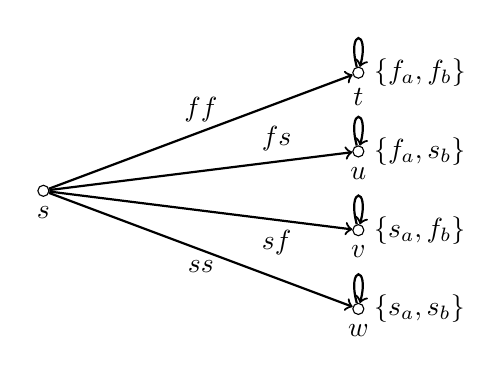
\begin{tikzpicture}
\node(-1) at (2,0) {};
\node[circle,draw=black, minimum size=4pt,inner sep=0pt,  label=below:{$s$}](1) at (0,0) {};
\node[circle,draw=black, minimum size=4pt,inner sep=0pt, , label=below:{$t$}, label = right:{$\{f_a, f_b\}$}](2) at (4,1.5) {};
\node[circle,draw=black, minimum size=4pt,inner sep=0pt, , label=below:{$u$}, label = right:{$\{f_a, s_b\}$}](3) at (4,0.5) {};
\node[circle,draw=black, minimum size=4pt,inner sep=0pt, , label=below:{$v$}, label = right:{$\{s_a, f_b\}$}](4) at (4,-0.5) {};
\node[circle,draw=black, minimum size=4pt,inner sep=0pt, , label=below:{$w$}, label = right:{$\{s_a, s_b\}$}](5) at (4,-1.5) {};

\draw [->,thick](1) to node[above,align=left] {$ff$} (2);
\draw [->,thick](1) to node[above,align=left, near end] {$fs$} (3);
\draw [->,thick](1) to node[below,align=left, near end] {$sf$} (4);
\draw [->,thick](1) to node[below,align=left] {$ss$} (5);
\draw [->,thick] (2) to [loop above]  (2);
\draw [->,thick] (3) to [loop above]  (3);
\draw [->,thick] (4) to [loop above]  (4);
\draw [->,thick] (5) to [loop above]  (5);
\end{tikzpicture}
}
\caption{CGS $\G$ for two agents and two actions. True atomic propositions represented in sets near corresponding states. For readability, self-loops labelled by all combinations of actions, are depicted as unlabelled loops.}
\label{fig::horror}
\end{figure} 
The CGS has five states, $s$, $t$, $u$, $v$, and $w$, and is defined over the set of two actions, $f$ for `folk horror', and $s$ for `sci-fi horror'. Propositional atoms correspond to the outcomes of Anna and Brita's actions with $f_a$ and $s_b$ being true in state $u$ meaning that Anna watches the folk horror film, and Brita watches the sci-fi horror film. 

Now, it is easy to verify that $\G,s \models \varphi$ since Anna can always choose action $f$ and thus let Brita play $f$ as well to reach her own goal. 
\end{example}

%\begin{example}
  %  Examples of CGSs are presented in Figure \ref{fig::exampleCGM}. In structure $\G_1$ we have two states $s$ and $t$, and the agents can transition between the two states if the execute the same actions. It is easy to verify that $\G_1,s \models \forall x \exists y \assign{x,y} p$ and $\G_1, s \models \forall x \assign{x,x} \lnot p$.
%\end{example}

   

\section{Relation to Other Formalisms}
\label{sec:expressivity}
In order to appreciate the richness of $\CSL$, we compare the logic to other related logics of strategic ability. In our comparison we will use two salient features of $\CSL$. First, the logic allows for \textit{arbitrary quantification prefixes for agents' actions}. This includes using the same strategy variable for different agents to capture \textit{strategy sharing}. The second special feature of $\CSL$ is the presence of \textit{explicit action labels} in its syntax.

\begin{definition}
    Let $\mathsf{L}_1$ and $\mathsf{L}_2$ be two languages, and let $\varphi \in \mathsf{L}_1$ and $\psi \in \mathsf{L}_2$. We call $\varphi$ and $\psi$ \emph{equivalent}, if for all CGSs $\G,s$ it holds that $\G,s \models \varphi$ if and only if $\G, s \models \psi$. 

    If for all $\varphi \in \mathsf{L}_1$ there exists and equivalent $\psi \in \mathsf{L}_2$, we say that $\mathsf{L}_2$ is \emph{at least as expressive as } $\mathsf{L}_1$ and write $\mathsf{L}_1 \leqslant \mathsf{L}_2$. We say that $\mathsf{L}_2$ is \emph{strictly more expressive than } $\mathsf{L}_2$ (denoted by $\mathsf{L}_1 < \mathsf{L}_2$) if $\mathsf{L}_1 \leqslant \mathsf{L}_2$ and $\mathsf{L}_2 \not \leqslant \mathsf{L}_1$.
\end{definition}

These two features of $\CSL$, arbitrary quantification prefixes and explicit actions, on their own are not unique in the landscape of logics for strategic reasoning. Thus, arbitrary quantification prefixes are a hallmark feature of the whole family of \textit{strategy logics} (see, e.g., \cite{mogavero10,belardinelli19}), to which $\CSL$ belongs. Indeed, $\CSL$ can be considered as a variation of the next-time fragment of \textit{strategy logic with simple goals} ($\mathsf{SL[SG]}$) \cite{belardinelli19}, which, in turn, is an extension of $\mathsf{ATL}$ \cite{alur02} with arbitrary quantification prefixes for agents' strategies. The idea to refer to action in the language has also been explored, with, perhaps, a prime example being $\mathsf{ATL}$ \textit{with explicit strategies} ($\mathsf{ATLES}$) \cite{walther07}. Another example of a logic with explicit actions is \textit{action logic} ($\mathsf{AL}$) \cite{borgo07}, which we will look at closer later in this section.

Even though both of the main features of $\CSL$ have been somewhat explored in the literature, to our knowledge, $\CSL$ is the first logic for strategic reasoning that combines \textit{both} of them. To further demonstrate the unique position of our logic in the landscape of related logics, we compare it to some known coalition logics. %explored in literature. 


%It is easy to show that $\CSL$ and $\mathsf{ATLES}$ are, expressivity-wise, incomparable. Indeed, in the former we can exploit arbitrary quantification prefix, and in the latter we have additional temporal expressivity. 

 %Moreover, $\CSL$ allows for actions of agents to be explicitly referenced in the logic language. These two features combined, i.e. arbitrary quantification prefixes and explicit action labels, make $\CSL$ quite unique in the landscape of the logics for strategic reasoning. 

 \paragraph{Coalition logic} The original \textit{coalition logic} ($\mathsf{CL}$) \cite{pauly02}, similarly to $\mathsf{ATL}$, allows only single alternation of quantifiers in coalitional modalities. Moreover, this quantification is implicit. Thus, $\mathsf{CL}$ extends the language of propositional logic with constructs $\langle \! \langle C \rangle \! \rangle \varphi$ that mean `there is a strategy for coalition $C$ to achieve $\varphi$ in the next step (whatever agents outside of the coalition do at the same time)'. 
 
 To introduce the semantics of $\mathsf{CL}$, we will denote the choice of actions by coalition $C \subseteq Agt$ with $|Agt| = n$ as $\sigma_C$, and denote $Agt \setminus C$ as $\overline{C}$. Finally, $\sigma_C \cup \sigma_{{\overline{C}}} \in \mathcal{D}$ is a decision. The semantics of $\langle \! \langle C \rangle \! \rangle \varphi$ for a given CGS $\G$ is then defined as 
  \begin{alignat*}{3}
        &\G,s \models \langle \! \langle C \rangle \! \rangle \varphi && \text{ iff } && \exists \sigma_C, \forall \sigma_{\overline{C}} : \G,t \models \varphi \\
        & && &&\text{ with } t \in S \text{ s.t. } \langle s, \sigma_C \cup \sigma_{\overline{C}}, t \rangle \in R.   
\end{alignat*}     
 
The translation from formulas $\mathsf{CL}$ to formulas of $\CSL$ can be done recursively using the following schema for coalitional modalities: 
$tr(\langle \! \langle C \rangle \! \rangle \varphi) \to \exists \vec x \forall \vec y \assign{\vec x, \vec y} tr(\varphi)$, 
where variables $\vec x$ (all different) quantify over actions of $C$, and $\vec y$ (all different) quantify over actions of $Agt \setminus C$. 

At the same time, one cannot refer to particular actions in $\mathsf{CL}$ formulas, as well as express sharing strategies between agents. We can exploit either of these features to show that $\CSL$ is strictly more expressive than $\mathsf{CL}$. 
Indeed, consider a $\CSL$ formula $\exists x \assign{x, x} \lnot p$ meaning that there is an action that \textit{both} agents 1 and 2 should use to reach a $\lnot p$-state. We can construct two CGSs that are indistinguishable by any $\mathsf{CL}$ formulas. At the same time,   $\exists x \assign{x, x} \lnot p$ will hold in one structure and be false in another. 

Consider two structures depicted in Figure \ref{fig::exampleCGM}. 

\begin{figure}[h!]
\centering
\scalebox{0.8}{
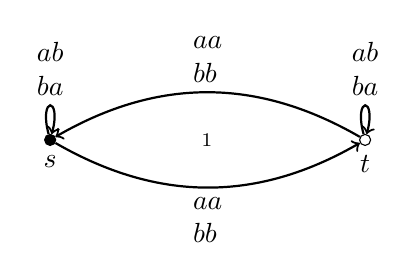
\begin{tikzpicture}
\node(-1) at (2,0) {$\G_1$};
\node[circle,draw=black, minimum size=4pt,inner sep=0pt, fill = black, label=below:{$s$}](1) at (0,0) {};
\node[circle,draw=black, minimum size=4pt,inner sep=0pt, , label=below:{$t$}](2) at (4,0) {};

\draw [->,thick](1) to [loop above] node[above, align=left] {$ab$\\$ba$} (1);
\draw [->,thick](1) to [bend right] node[below,align=left] {$aa$\\$bb$} (2);
\draw [->,thick] (2) to [bend right] node[above,align=left] {$aa$\\$bb$} (1);
\draw [->,thick] (2) to [loop above] node[above,align=left] {$ab$\\$ba$} (2);
\end{tikzpicture}
\hspace{10mm}
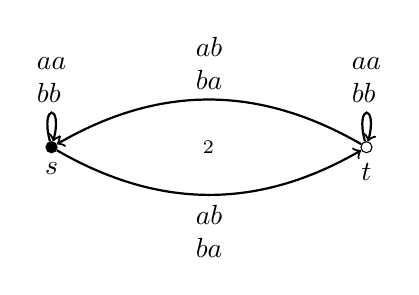
\begin{tikzpicture}
\node(-1) at (2,0) {$\G_2$};
\node[circle,draw=black, minimum size=4pt,inner sep=0pt, fill = black, label=below:{$s$}](1) at (0,0) {};
\node[circle,draw=black, minimum size=4pt,inner sep=0pt, , label=below:{$t$}](2) at (4,0) {};

\draw [->,thick] (1) to [loop above] node[above, align=left] {$aa$\\$bb$} (1);
\draw [->,thick](1) to [bend right] node[below,align=left] {$ab$\\$ba$} (2);
\draw [->,thick] (2) to [bend right] node[above,align=left] {$ab$\\$ba$} (1);
\draw [->,thick] (2) to [loop above] node[above,align=left] {$aa$\\$bb$} (2);
\end{tikzpicture}
}
\caption{CGSs $\G_1$ and $\G_2$ for two agents and two actions. Propositional variable $p$ is true in black states.}
\label{fig::exampleCGM}
\end{figure} 
It is easy to see that $\G_1,s$ and $\G_2,s$ cannot be distinguished by any $\mathsf{CL}$ formula\footnote{These structures are, in fact, bisimilar \cite{agotnes07}, and hence satisfy the same formulas of $\mathsf{CL}$ and $\mathsf{ATL}$. The discussion of bisimulations for all the logics we mention is, however, beyond the scope of this paper, and we leave it for future work.}. Indeed, both structures agree on the valuation of propositional variable $p$ in corresponding states. Moreover, none of the agents, 1 and 2, can on their own force a transition from state $s$ to state $t$. At the same time, the grand coalition $\{1,2\}$ can match any transition in one structure with a transition with the same effect in the other structure. %force any transition in both structures. 
Now, we can verify that $\G_1,s \models \exists x \assign{x, x} \lnot p$ and $\G_2,s \not \models \exists x \assign{x, x} \lnot p$. For the case of  $\G_1,s \models \exists x \assign{x, x} \lnot p$, it is enough to assign action $a$ to $x$ to have $\G_1,s \models \assign{a, a} \lnot p$. To make $\G_2,s \not \models \exists x \assign{x, x} \lnot p$ hold, one needs to provide an action that once executed by both agents will force the transition to state $t$. It is easy to see that there is no such an action in $\G_2,s$.

Having the translation from $\mathsf{CL}$ to $\CSL$ on the one hand, and the indistinguishability result on the other, we hence conclude that $\CSL$ is \textit{strictly more expressive} than $\mathsf{CL}$.

\begin{proposition}
\label{prop:cslVScl}
    $\mathsf{CL} < \CSL$.
\end{proposition}

\paragraph{Conditional strategic reasoning and socially friendly coalition logic} With the expressive power of $\CSL$ we can go much further than the classic $\mathsf{CL}$. In particular, we can express in our logic such interesting coalition logics like \textit{logic for conditional strategic reasoning} ($\mathsf{ConStR}$) \cite{goranko22}, \textit{socially friendly coalition logic} ($\mathsf{SFCL}$) \cite{goranko18}, and \textit{group protecting coalition logic} ($\mathsf{GPCL}$)  \cite{goranko18}. 

Presenting the semantics of the aforementioned logic is beyond the scope of this paper. However, we would like to point out that all of the logics can be captured by \textit{basic strategy logic} ($\mathsf{BSL}$) \cite{goranko23}, which is a variant of $\mathsf{SL}$ where each agent has her own associated strategy variable. Differently from $\CSL$, $\BSL$ allows for all standard temporal modalities like `ne\textsf{X}t', `\textsf{U}ntil' and `\textsf{G}lobally (or Forever)'. At the same time, $\BSL$ does not allow for variable sharing and does not explicitly refer to actions or strategies. Moreover, it is conjectured \cite{goranko23} that $\BSL$ does not have a recursive axiomatisation, while $\CSL$ has a finitary complete axiomatisation (see Section \ref{sec:axiom}).

Translations of all coalition logics introduced in this paragraph into formulas of $\mathsf{BSL}$ are presented in \cite{goranko23}, where it is also claimed that $\mathsf{BSL}$ is strictly more expressive than all the aforementioned logics. The translation does not employ any temporal features of $\mathsf{BSL}$ apart from `ne\textsf{X}t', and thus the same translation also works for $\CSL$. Moreover, we can use either strategy sharing or explicit actions to argue that $\CSL$ is strictly more expressive than the considered coalition logics.

%For the sake of an example, 
As an example,
we provide an argument for $\mathsf{SFCL}$ that extends the language of propositional logic with constructs $\langle \! \langle  C \rangle \! \rangle (\varphi;\psi_1,...,\psi_k)$ meaning that `coalition $C$ can achieve $\varphi$ while also enabling $\overline{C}$ to achieve any of $\psi_1,...,\psi_k$ (via a suitable joint action)'. 

Formally, the semantics is defined as 
  \begin{alignat*}{3}
        &\G,s \models \langle \! \langle C \rangle \! \rangle (\varphi; \psi_1, ..., \psi_k) && \text{ iff } && \exists \sigma_C (\forall \sigma_{\overline{C}} : \G,t \models \varphi \text{ and } \forall \psi_i, \exists  \sigma_{\overline{C}}:\\
         & && &&\G_u \models \psi) \text{ with } t,u \in S \text{ s.t. }\\
        & && &&\langle s, \sigma_C \cup \sigma_{\overline{C}}, w \rangle \in R \text{ and } w \in \{t,u\}.   
\end{alignat*}   

Now, let us have another look at CGSs in Figure \ref{fig::exampleCGM}. Recall that these structures are distinguished by the $\CSL$ formula $\exists x \assign{x,x} \lnot p$. We claim that no formula of $\mathsf{SFCL}$ can distinguish $\G_1,s$ from $\G_2,s$. An informal sketch of the induction-based argument is as follows. For purely propositional formulas it is clear that $\G_1,w$ and $\G_2,w$ with $w\in \{s,t\}$ satisfy the same formulas. Now, let us consider socially-friendly coalitional modalities $\langle \! \langle  C \rangle \! \rangle (\varphi;\psi_1,...,\psi_k)$ For the case of grand coalition $C = \{1,2\}$, it is easy to verify that any move in $\G_1,w$ can be matched by a corresponding move $\G_2,w$ to satisfy $\varphi$. Clearly, these transitions will require different actions by agents, but since we do not have access to action labels in $\mathsf{SFCL}$, we are not able to spot the difference. 

For the case of single agents, observe that yet again, every choice of, let's say, agent 1 in one structure can be matched by a choice in the other structure to the same effect. Indeed, whatever agent 1 chooses in $\G_1, s$, $a$ or $b$, she can only satisfy some $\varphi$ that holds in both states $s$ and $t$ (due to the fact that the outcome is determined by what agent 2 chooses as well). Similarly in $\G_2, s$. Now, goals $\psi_i$ of agent 2 can either be satisfied in state $s$, state $t$, or both states. Hence, by the construction of CGSs, in both $\G_1$ and $\G_2$ for each choice of agent 1, agent 2 has an action to either stay in the current state or force the transition to another state. That the outcome of the corresponding transitions satisfy $\psi_i$ follows from the induction hypothesis. 

\begin{proposition}
    $\mathsf{ConStR} < \CSL$, $\mathsf{SFCL} < \CSL$, $\mathsf{GPCL} < \CSL$.
\end{proposition}

\paragraph{Action logic} 

A perhaps most relevant to $\CSL$ coalition logic in the literature is \textit{action logic} ($\mathsf{AL}$) \cite{borgo07}, which is a fragment of \textit{multi-agent PDL with quantificaiton} ($\mathsf{mPDLQ}$) \cite{borgo05}. $\mathsf{AL}$ extends the language of propositional logic with so-called \textit{modality markers} $[M]$, which are, essentially, prefixes of size $|Agt| = n$, each element of which can either be a quantifier $Q_i x_i$ with $Q_i \in \{\forall, \exists\}$ or an explicit action \cite{borgo05,borgo05b}. An important feature here is that \textit{there are no repeating variables in modality markers}. Finally, to the best of our knowledge, there is no axiomatisation of  $\mathsf{AL}$.

Interpreted on concurrent game structures, modality markers have the following semantics:
  \begin{alignat*}{3}
        &\G,s \models [M] \varphi && \text{ iff } && \text{ for all } x_1, ...., x_m \text{ with } \exists x_i \in M, \exists a_i \in \Ac \text{ s.t. }\\
        & && &&\langle s, A, s'\rangle \in R \text{ and } \G,s'\models \varphi,\\ & && &&\text{ for all } A \text{ s.t. } a_1, ..., a_m \sqsubseteq A.  
\end{alignat*}    
Intuitively, $\G,s \models [M] \varphi$ holds if and only if there is an assignment of actions to all existentially quantified variables in modality marker $M$ such that no matter which actions are explicit in $M$ and which actions are assigned to the universally quantified variables, the outcome state satisfies $\varphi$. Observe that this is in line with the semantics of $\mathsf{CL}$ as we basically choose actions for a coalition (existentially quantified variables) and verify $\psi$ in all possible outcomes given this choice. 

It is easy to see that formulas $[M]\varphi$ of $\mathsf{AL}$ can be trivially translated into formulas of $\CSL$ of the form $Q_1 x_1, .., Q_n x_m \assign{t_1, ..., t_n} \varphi$, where $t_i := x_i$ if there is a quantifier in position $i$ in the modality marker, and $t_i:= a_i$ if there is action $a_i$ in the $i$th posiiton in the modality marker. Also recall that $\mathsf{AL}$ does not allow for sharing strategies (while $\CSL$ does), i.e. all $x_1, ..., x_m$ in the modality marker are unique. 

To show that $\CSL$ is more expressive than $\mathsf{AL}$, we need to prove the following lemma. %approach the relative expressivity of $\CSL$ and $\mathsf{AL}$ formally, we prove the following lemma. 

\begin{lemma}
\label{lemma:exp}
    $\mathsf{AL}$ is not at least as expressive as $\CSL$.
\end{lemma}

\begin{proof}
    Consider $\exists x \assign{x, x} \lnot p \in \CSL$, and assume towards a contradiction that there is an equivalent $\varphi \in \mathsf{AL}$. Since we have a countably infinite set of constants $\mathcal{C}$ (and hence actions) at our disposal  and due to the fact that $\varphi$ is finite, we can assume that there are actions $a$ and $b$ that do not appear explicitly in $\varphi$. 

Now, consider two concurrent game structures defined over two agents and two actions in Figure \ref{fig::exampleCGM}. As we have already seen in our argument for Proposition \ref{prop:cslVScl}, $\G_1,s \models \exists x \assign{x, x} \lnot p$ and $\G_2,s \not \models \exists x \assign{x, x} \lnot p$. What is left to show is that $\varphi$ cannot distinguish the two structures, i.e. $\G_1,s \models \varphi$ if and only if $\G_2, s \models \varphi$.

    The proof is by induction on the complexity of $\varphi$. As the \textit{Base Case}, by the construction of the structures we have that $\G_1,w \models p$ if and only if $\G_2,w \models p$ for $w \in \{s,t\}$ and all $p \in \Ap$. 

    \textit{Induction Hypothesis.} $\G_1,w \models \psi$ if and only if $\G_2, w \models \psi$  for $w \in \{s,t\}$ and for all strict subformulas $\psi$ of $\varphi$.
    
    Boolean cases follow straightforwardly by the induction hypothesis. What is left is the case of modality markers. 

   \textit{Case } $\varphi := [M]\psi$. First, recall that we assume that actions $a$ and $b$ do not appear explicitly in $\varphi$. It is enough to verify four forms of modality markers corresponding to all possible combinations of quantifiers over actions for two agents. Let $\varphi = [\exists x, \exists y] \psi$. It is easy to see that  $\G_1,w \models [\exists x, \exists y] \psi$ if and only if $\G_2,w \models [\exists x, \exists y] \psi$ as in both CGSs the grand coalition of agents $\{1,2\}$ has the full control over which transitions to force. Hence, each move in $\G_1,w$ to a $\psi$-state $v \in \{s,t\}$ can be matched by a move in  $\G_2,w$ to the same $\psi$-state $v$, where we will have $\G_1,v \models \psi$ if and only if $\G_2,v \models \psi$ by the induction hypothesis. 
   The remaining cases for modality markers can be shown similarly.
\end{proof}

Having the translation from $\mathsf{AL}$ to $\CSL$ on the one hand, and Lemma \ref{lemma:exp} on the other, we can conclude that $\CSL$ is strictly more expressive than $\mathsf{AL}$.

\begin{proposition}
\label{alVScsl}
    $\mathsf{AL} < \CSL$.
\end{proposition}



\paragraph{The expressivity landscape}
In this section we have explored the relationship between $\CSL$ and other notable coalition logics from the literature. The overall expressivity landscape of the considered logics is presented in Figure \ref{fig:expressivity}.

\begin{figure}[h!]
\centering
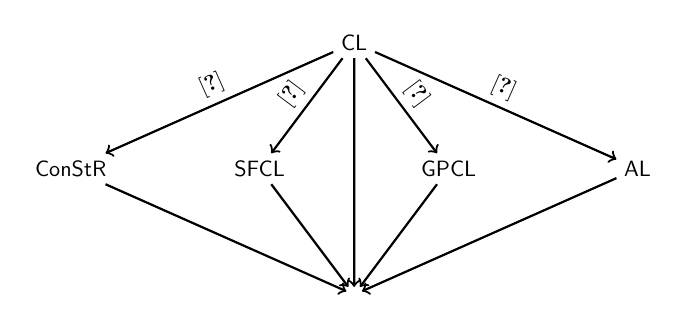
\begin{tikzpicture}[scale=0.8, transform shape]
\node (constr) at (0,0) {$\mathsf{ConStR}$};
\node (sfcl) at (3,0) {$\mathsf{SFCL}$};
\node (gpcl) at (6,0) {$\mathsf{GPCL}$};
\node (al) at (9,0) {$\mathsf{AL}$};
\node (csl) at (4.5,-2) {$\CSL$};
\node (cl) at (4.5,2) {$\mathsf{CL}$};

\draw[thick,<-] (constr) to node[sloped, anchor=center, above] {\cite{goranko22}} (cl);
\draw[thick,<-] (sfcl) to node[sloped, anchor=center, above] {\cite{goranko18}} (cl);
\draw[thick,<-] (gpcl) to node[sloped, anchor=center, above] {\cite{goranko18}} (cl);
\draw[thick,<-] (al) to node[sloped, anchor=center, above] {\cite{borgo07}} (cl);
\draw[thick,<-] (csl) to (cl);
\draw[thick,<-] (csl) to (constr);
\draw[thick,<-] (csl) to (sfcl);
\draw[thick,<-] (csl) to (gpcl);
\draw[thick,<-] (csl) to (al);
\end{tikzpicture}
\caption{Overview of the expressivity results. An arrow from $\mathsf{L}_1$ to $\mathsf{L}_2$ means $\mathsf{L}_1 <\mathsf{L}_2$. Arrows labelled with a citation represent results from the literature. Arrows without labels are new results.}
\label{fig:expressivity}
\end{figure}

\section{Model checking}
\label{sec:mc}
%Now we turn to the complexity of the model checking problem for $\CSL$, and show that despite $\CSL$ being quite expressive, its model checking can be done in polynomial time.
Now we turn to the complexity of the model checking problem for $\CSL$, and show that %the high expressivity of $\CSL$ comes at a price: its model checking procedure 
it is \textit{PSPACE}-complete.

\begin{definition}
    Let $\G = \tuple{n,\Ac, \mathcal{D}, S,R, \mathcal{V} }$ be a finite CGS, $s \in S$, and closed formula $\varphi \in \CSL$ constructed over a signature of $\G$. The \emph{local model checking problem} for $\CSL$ consists in computing whether $\G, s \models \varphi$.
\end{definition}


\iffalse
Before providing the model-checking algorithm, we need a given formula of $\CSL$ to conform to a certain form. 

\begin{definition}
    Let $\varphi$ be a formula of $\CSL$. Then \emph{width} of $\varphi$, denoted $w(\varphi)$, is a maximal number of free variables in subformulae of $\varphi$.
\end{definition}

With the next lemma we show that each formula has an equivalent formula with width equal to $n$, where $n$ is the number of agents. Intuitively, this means that for each assignment $\assign{t_1, ..., t_n}$ it is enough to consider only $n$ quantifiers.

\begin{lemma}
    For each $\varphi \in \CSL$, there is an equivalent $\psi \in \CSL$ with $w(\psi) = n$.
\end{lemma}

\begin{proof}
    
\end{proof}

\begin{theorem}
    The local model checking problem for $\CSL$ is $P$-complete.
\end{theorem}

\begin{proof}
Consider Algorithm \ref{cslMC}.

\begin{breakablealgorithm}
	\caption{An algorithm for model checking $\CSL$} \label{cslMC} 
	%\small
 %\footnotesize
	\begin{algorithmic}[1] 		
		\Procedure{MC}{$\G, s, \varphi$}		
      \Case {$\varphi = p$}
            \State{\textbf{return} $s \in \mathcal{V}(p)$}
        \EndCase
        \Case {$\varphi = \lnot \psi$}
            \State{\textbf{return}  not $\textsc{MC} (\G, s, \psi)$}
       \EndCase
       \Case {$\varphi = \psi \lor \chi$}
            \State{\textbf{return} $\textsc{MC} (\G,s,\psi)$ or  $\textsc{MC} (\G,s,\chi)$}
        \EndCase
       \Case {$\varphi = \assign{a_1,...,a_n} \psi$}
       \If {$\tuple{s, a_1, ..., a_n, t} \in R$ for some $t\in S$}
            \State{\textbf{return} $\textsc{MC} (\G, t, \psi)$}
        \Else
            \State{\textbf{return} \textit{false}}
       \EndIf
            \State{\textbf{return} $\textsc{MC} (\G,s,\psi)$ or  $\textsc{MC} (\G,s,\chi)$}
        \EndCase
        \Case{$\varphi = \forall x \psi$}
        \ForAll {$a \in \Ac$}
            \If{not $\textsc{MC} (\G,s,\psi[a/x])$}
                \State{\textbf{return} \textit{false}}
            \EndIf
        \EndFor
        \State{\textbf{return} \textit{true}}
        \EndCase
   \EndProcedure
	\end{algorithmic}
\end{breakablealgorithm}
The termination of the algorithm follows from the finiteness of $\G$ and $\varphi$. Correctness follows from the fact that the algorithm clearly imitates the definition of the semantics of $\CSL$. 

In the worst case, i.e. the case of $\forall x \psi$, we call the algorithm for $|\varphi|$ times with each call having $|\Ac|$ iterations of the for-loop. We run this for $|\varphi|$ subformulas of $\varphi$,  and hence the overall the running time of the algorithm is bounded by $\mathcal{O} (|\varphi|^2 \cdot |\Ac|)$.

The lower bound is obtained from the fact that $\mathsf{CL}$ is translatable into $\CSL$ (Section \ref{sec:expressivity}) and $P$-completeness of the model checking for coalition logic \cite{bulling010}.
\end{proof}
\fi

\begin{theorem}
    The model checking problem for $\CSL$ is PSPACE-complete.
\end{theorem}

\begin{proof}
To show that the model checking problem for $\CSL$ is in \textit{PSPACE}, we provide an alternating recursive Algorithm \ref{cslMC} that takes as an input a finite CGS $\G$, state of the CGS $s$, and a closed formula $\varphi$. The formula $\varphi$ is provided in negation normal form (NNF), i.e. in equivalent rewriting, where all negations are pushed inside and appear only in front of propositional variables. To convert $\varphi$ into the equivalent NNF formula, we can use propositional equivalences, interdefinability of quantifiers, and the validity  $\neg \assign{\Vec{t}}\varphi \leftrightarrow \assign{\vec{t }}\neg \varphi$. The size of a formula in NNF is at most linear in the size of the original formula.

\begin{breakablealgorithm}
	\caption{An algorithm for model checking $\CSL$} \label{cslMC} 
	%\small
 %\footnotesize
	\begin{algorithmic}[1] 		
		\Procedure{MC}{$\G, s, \varphi$}		
      \Case {$\varphi = p$}
            \State{\textbf{return} $s \in \mathcal{V}(p)$}
        \EndCase
          \Case {$\varphi = \lnot p$}
            \State{\textbf{return} not $s \in \mathcal{V}(p)$}
        \EndCase
       \Case {$\varphi = \psi \lor \chi$}
            \State{\textbf{guess} $\theta \in \{\psi, \chi\}$  }
            \State{\textbf{return} $\textsc{MC} (\G,s,\theta)$}
        \EndCase
               \Case {$\varphi = \psi \land \chi$}
            \State{\textbf{universally choose} $\theta \in \{\psi, \chi\}$  }
            \State{\textbf{return} $\textsc{MC} (\G,s,\theta)$}
        \EndCase
       \Case {$\varphi = \assign{a_1,...,a_n} \psi$}
       \State{\textbf{guess} $t \in S$ such that   $\tuple{s, a_1, ..., a_n, t} \in R$}
       \State{\textbf{return} $\textsc{MC} (\G, t, \psi)$}
       %%\If {$\tuple{s, a_1, ..., a_n, t} \in R$ for some $t\in S$}
            %\State{\textbf{return} $\textsc{MC} (\G, t, \psi)$}
        %\Else
       %     \State{\textbf{return} \textit{false}}
      % \EndIf
       %     \State{\textbf{return} $\textsc{MC} (\G,s,\psi)$ or  $\textsc{MC} (\G,s,\chi)$}
        \EndCase
         \Case{$\varphi = \exists x \psi$}
        \State{\textbf{guess} $a \in \Ac$  }
        \State{\textbf{return} $\textsc{MC} (\G,s,\psi[a/x])$}
        %\ForAll {$a \in \Ac$}
            %\If{not $\textsc{MC} (\G,s,\psi[a/x])$}
              %  \State{\textbf{return} \textit{false}}
           % \EndIf
        %\EndFor
       % \State{\textbf{return} \textit{true}}
        \EndCase
        \Case{$\varphi = \forall x \psi$}
        \State{\textbf{universally choose} $a \in \Ac$  }
        \State{\textbf{return} $\textsc{MC} (\G,s,\psi[a/x])$}
        %\ForAll {$a \in \Ac$}
            %\If{not $\textsc{MC} (\G,s,\psi[a/x])$}
              %  \State{\textbf{return} \textit{false}}
           % \EndIf
        %\EndFor
       % \State{\textbf{return} \textit{true}}
        \EndCase
   \EndProcedure
	\end{algorithmic}
\end{breakablealgorithm}

The correctness of the algorithm follows from the definition of the semantics. Its termination follows from the fact that every recursive call is run on a subformula of smaller size. Moreover, each call of the algorithm takes at most polynomial time, and hence it is in \textit{APTIME}. From the fact that \textit{APTIME} = \textit{PSPACE} \cite{alternation}, we conclude that the model checking problem for $\CSL$ is in \textit{PSPACE}.

    The hardness is shown by the reduction from the classic satisfiability of quantified Boolean formulas (QBF). For a given QBF $\Psi:=Q_1 p_1 ... Q_n p_n \psi (p_1, ..., p_n)$ with $Q_i \in \{\forall, \exists\}$, the problem consists in determining whether $\Psi$ is true. Without loss of generality, we assume that in $\Psi$ each variable is quantified only once.

    Given a QBF $\Psi:=Q_1 p_1 ... Q_n p_n \psi (p_1, ..., p_n)$, we construct a CGS over one agent $\G = \langle 1, \Ac, \mathcal{D}, S, R, \mathcal{V} \rangle$, where $\Ac = \{a_1, ..., a_n\}$, $\mathcal{D} = \Ac$, $S = \{s, s_1, ..., s_n\}$, $R = \{\langle s, a_i, s_i\rangle \mid i \in \{1,...,n\}\} \cup \{\langle s_i, a_j, s_i \rangle \mid i,j \in \{1,...,n\}\}$, and $\mathcal{V}(p_i) = \{s_i\}$. Intuitively, CGS $\G$ has a starting state $s$ and a state $s_i$ for each $p_i$. The agent can reach $s_i$ from $s$ by executing action $a_i$, and all the transitions from $s_i$'s are self-loops.

    The translation from the QBF $\Psi$ into a formula $\varphi$ of $\CSL$ is done recursively as follows: 
    \begin{align*}
    \varphi_0 &:= \psi(\assign{x_1} p_1, ..., \assign{x_n}p_n) \\
    \varphi_k &:=
    \begin{cases}
        \forall x_k \varphi_{k-1} &\text{if } Q_k = \forall\\ 
        \exists x_k \varphi_{k-1} &\text{if } Q_k = \exists\\
    \end{cases}\\
\varphi &:= \varphi_n
\end{align*}
To see that 
$$Q_1 p_1 ... Q_n p_n \psi (p_1, ..., p_n) \text{ is satisfiable iff } \G,s \models \varphi$$
it is enough to notice that setting the truth-value of propositional variable $p_i$ to 1 is modelled by reachability via action $a_i$ of the state $s_i$, where $p_i$ holds. Quantifiers are modelled directly as quantifiers over the agent's actions. 

As an example, consider a QBF $\forall p_2 \exists p_1 \exists p_3 (p_1 \to p_2) \land p_3$, which is clearly satisfiable with $p_1 = 0$ and $p_3 = 1$. The formula is translated into the formula of $\CSL$: $\forall x_2 \exists x_1  \exists x_3 (\assign{x_1}p_1 \to \assign{x_2}p_2) \land \assign{x_3}p_3$. The corresponding CGS is presented in Figure \ref{fig::hardness}, and it is easy to verify that $\G,s \models \forall x_2 \exists x_1  \exists x_3 (\assign{x_1}p_1 \to \assign{x_2}p_2) \land \assign{x_3}p_3$.
\end{proof}
\begin{figure}[h!]
\centering
\scalebox{0.9}{
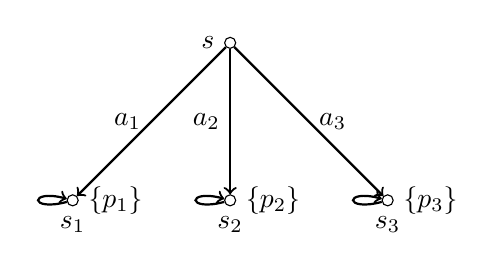
\begin{tikzpicture}
\node(-1) at (2,0) {};
\node[circle,draw=black, minimum size=4pt,inner sep=0pt,  label=left:{$s$}](1) at (0,0) {};
\node[circle,draw=black, minimum size=4pt,inner sep=0pt, , label=below:{$s_1$}, label = right:{$\{p_1\}$}](2) at (-2,-2) {};
\node[circle,draw=black, minimum size=4pt,inner sep=0pt, , label=below:{$s_2$}, label = right:{$\{p_2\}$}](3) at (0,-2) {};
\node[circle,draw=black, minimum size=4pt,inner sep=0pt, , label=below:{$s_3$}, label = right:{$\{p_3\}$}](4) at (2,-2) {};

\draw [->,thick](1) to node[left,align=left] {$a_1$} (2);
\draw [->,thick](1) to node[left,align=left] {$a_2$} (3);
\draw [->,thick](1) to node[right,align=left] {$a_3$} (4);
\draw [->,thick] (2) to [loop left]  (2);
\draw [->,thick] (3) to [loop left]  (3);
\draw [->,thick] (4) to [loop left]  (4);
\end{tikzpicture}
}
\caption{CGS $\G$ for a single agent. Labels for self-loops are omitted for readability.}
\label{fig::hardness}
\end{figure} 

\begin{remark}
    The complexity of the model checking problem for a related \textit{strategy logic with simple goals} ($\mathsf{SL[SG]}$) is known to be $P$-complete \cite{belardinelli19}. 
This is due to the fact that in $\mathsf{SL[SG]}$ the quantification prefix and the operators for assigning strategies to agents always go together. Hence, for example, the $\CSL$ formula over two agents $\theta:=\forall x \exists y \forall z (\assign{z,x} \varphi \land \assign{z,y} \psi \land \assign{x,z}\chi)$ cannot be expressed in the language of $\mathsf{SL[SG]}$. The higher complexity of $\CSL$ stems from the fact that quantifiers and strategy assignments are less rigid than in $\mathsf{SL[SG]}$, and thus $\CSL$ is closer to the full $\mathsf{SL}$ in this regard. 
\end{remark}




\section{Proof theory}
\label{sec:axiom}

\subsection{Context}
Perhaps the best-known results in the field are complete axiomatisations of $\mathsf{CL}$ \cite{pauly02,goranko13} and $\mathsf{ATL}$ \cite{goranko06} (see \cite{walther06,goranko09} for more constructive approaches to the construction of the canonical model). Other completeness results include axiomatisations for logics based on $\mathsf{CL}$ and $\mathsf{ATL}$, like already mentioned $\mathsf{SFCL}$ \cite{goranko18}, $\mathsf{ATLES}$ \cite{walther07}, as well as \textit{epistemic} $\mathsf{CL}$ \cite{agotnes19}, \textit{resource-bounded} $\mathsf{CL}$\cite{alechina11}, \textit{resource-bounded} $\mathsf{ATL}$ \cite{nguyen18}, and $\mathsf{ATL}$ \textit{with finitely bounded semantics} \cite{goranko19}, to name a few.

In the context of strategy logics, we have quite an opposite picture. Since the inception of $\mathsf{SL}$ \cite{mogavero10}, its completeness has been an open problem. Indeed, the satisfiability problem for the original $\mathsf{SL}$ is $\Sigma^1_1$-hard \cite{mogavero16}, which implies that $\mathsf{SL}$ is not recursively axiomatisable. This does not rule out, though, the existentence of an \textit{infinitary} axiomatisation.
A fragment of $\mathsf{SL}$, called \textit{one-goal} $\mathsf{SL}$ ($\mathsf{SL[1G]}$), has a decidable satisfiability problem so there is a hope of having a proof system for it. However, $\mathsf{SL[1G]}$ subsumes $\mathsf{ATL}^\ast$, and providing a complete axiomatisation of the latter is yet another long-standing open problem. 

The lack of axiomatisations of \textit{any} (fragment of) $\mathsf{SL}$ can be traced back to the two main features of the logic: quantification over strategies and arbitrary quantification prefixes. %To understand these nuances of $\mathsf{SL}$ better, we need the following defintion.

%\begin{definition}
%    Let $\G = \tuple{n,\Ac, \mathcal{D}, S,R, \mathcal{V} }$ be a CGS. A \emph{(memoryless) strategy} for an agent $i \in n$ is a function $\sigma_i: S \to \Ac$. The set of all strategies of all agents is denoted as $\Sigma (\G)$. An \emph{assignment} is a function $\chi: \V \cup n \to \Sigma (\G)$ that assigns strategies from $\Sigma (\G)$ to each agent and each variable.
%\end{definition}

%The language of $\mathsf{SL}$ extends the language of \textit{linear temporal logic} ($\mathsf{LTL})$ with constructs for quantification over strategies $\exists x \varphi$ and for binding agents to strategies $(x,i) \varphi$. The latter means `agent $i$ can achieve $\varphi$ by using strategy assigned to $x$'. The semantics of $\mathsf{SL}$ is defined relative to a given assignment $\chi$:
   % \begin{alignat*}{3}
     %   &\G,s\models_\chi \exists x \varphi &&\text{ iff } &&\exists \sigma_i \text{ for all agents } i \text{ bound to } x: \G,s\models_{\chi_{\sigma_i}^x} \varphi\\
     %   &\G,s\models_\chi (x,i) \varphi &&\text{ iff } && \G,s\models_{\chi_{\chi(x)}^i} \varphi
    %\end{alignat*}
%In the semantics, $\chi_{\sigma_i}^x$ stands for a variant of $\chi$ such that variable $x$ is assigned strategy $\sigma_i$ (and everything else is the same), and $\chi_{\chi(x)}^i$ stands for a variant  of $\chi$, where agent $i$ is assigned the strategy associated with variable $x$ (and everything else is the same).

%Having these definitions in mind, it is easy to note that, firstly, the quantification prefix of $\mathsf{SL}$ formulas can be arbitrary. 
Indeed, arbitrary alternation of quantifiers in $\mathsf{SL}$ is quite different from the fixed quantification prefix of $\mathsf{CL}$ and $\mathsf{ATL}$ that allow only prefixes $\exists \forall$ and $\forall \exists$. Secondly, quantification over strategies\footnote{A \emph{(memoryless) strategy} for an agent $i \in n$ is a function $\sigma_i: S \to \Ac$.}  in $\mathsf{SL}$ is essentially a second-order quantification over functions. We believe that these two features combined are the root cause of the fact that no complete axiomatisations of (fragments of) $\mathsf{SL}$ %or its fragments 
have been proposed so far. 

In $\CSL$ we focus on arbitrary quantification prefixes. To solve this sub-problem, we consider only ne$\mathsf{X}$t-time modalities $\assign{t_1,...,t_n} \varphi$ and focus on the immediate outcomes of agents' choices. Other temporal modalities, like $\mathsf{U}$ntil and $\mathsf{E}$ventually would require a more complicated construction as their truth values depend on the whole computation paths rather than just the next step (see \cite{goranko06} on how to deal with them in the context of $\mathsf{ATL}$). Such a design choice allows us, in particular, to consider quantification over actions rather than strategies. %(see the semantics of $\CSL$ and $\mathsf{SL}$ for comparison). 
Hence, quantification in $\CSL$ is a first-order quantification, instead of the second-order quantification of $\mathsf{SL}$. The relation between various fragments of $\mathsf{SL}$ and the corresponding induced fragments of $\mathsf{FOL}$ is explored in \cite{mogavero15}.

In the completeness proof in the following section, we take as inspiration the completeness proof for \textit{first-order modal logic} ($\mathsf{FOML}$) with constant domains \cite{Garson1984}. Our construction is quite different, though, as in $\mathsf{FOML}$ variables appear in $n$-ary predicates, and in $\CSL$ variables are placeholders for transition labels.  

\subsection{A Sound and Complete Axiomatisation of $\CSL$}

\begin{definition}
    The \emph{axiom system} for $\CSL$ consist of the following axiom schemata and rules, where $\vec{t}=t_1,\ldots,t_n$ for $n\geq 1$, and each $t_i$ is either a variable or a constant, and likewise for $t$.
    $$
\begin{array}{c
%@{\qquad}
l}

    \mathsf{PC}  & \text{Every propositional tautology}  
  \\
     \mathsf{K} & ( \assign{\vec{t}} \varphi \land \assign{\vec{t}}\psi) \leftrightarrow \assign{\vec{t}}(\varphi \land \psi )
   \\
   \mathsf{\mathsf{N} } & \neg \assign{\Vec{t}}\varphi \leftrightarrow \assign{\vec{t }}\neg \varphi 

   \\
   \mathsf{E} & \forall x \varphi \to \varphi[t/x]
\\
\mathsf{B} & \forall x \assign{\vec t} \varphi \imp \assign{\vec t} \forall x \varphi \text{, where each } t_i \text{ is different from $x$} %\qquad   % x\neq t_i \text{ for all $i\leq n$} 
\\
\mathsf{MP} & \text{From } \varphi, \varphi \to \psi, \text{ infer } \psi
\\
\mathsf{Nec} & \text{From } \varphi, \text{ infer } \assign{\vec t }\varphi
\\
\mathsf{Gen} & \text{From } \varphi\to \psi[t/x] , \text{ infer } \varphi\to \forall x \psi, \text{ if $t$  does not appear in $\varphi$}
\end{array}
$$
\iffalse
\begin{tabular}{p{0.33\textwidth} p{0.33\textwidth} p{0.33\textwidth}}

   \begin{prooftree}
       \AxiomC{$\varphi$}\LeftLabel{$\mathsf{MP}$}
       \AxiomC{$\varphi \to \psi$}
       \BinaryInfC{$\psi$}
   \end{prooftree} 
   &  
  \begin{prooftree}
       \AxiomC{$\varphi$}\LeftLabel{$\mathsf{Nec}$}
         \UnaryInfC{$\assign{\vec t }\varphi $}
   \end{prooftree} 
   
     &  \begin{prooftree}
       \AxiomC{$\varphi\to \psi $}\RightLabel{$x\notin \FV(\varphi  )$}\LeftLabel{$\mathsf{Gen}$}
        \UnaryInfC{$\varphi\to \forall x \psi$}
   \end{prooftree} 

     
\end{tabular}
\fi
\noindent An axiomatic derivation $\pi$ is a finite sequence of formulae $\varphi_1,\ldots, \varphi_m$ where for each $i\leq m$:  either $\varphi_i$ is an instance of one of the axiom schemata of $\CSL$, or it is obtained by some preceding formulae in the sequence using rules $\mathsf{MP}$, $\mathsf{Nec}$, or $\mathsf{Gen}$.
We write   $\vdash\varphi$ and we say that  $\varphi$ is \emph{CSL derivable} (or simply derivable)  iff there is a derivation $\pi$ whose last element is $\varphi$. Given a set of formulae $X$, we write $X \vdash \varphi$ iff there is a finite subset $Y $ of $X$ such that %$\vdash_\CSL \bigwedge Y \imp \varphi$. 
$\vdash \bigwedge Y \imp \varphi$.
\end{definition}


We will freely use the following proposition in the rest of the paper. Its proof is relatively standard, and we omit it for brevity. 

\begin{proposition}\label{prop.first}
    The following formulae are $\CSL$ derivable, where $\vec{t}=t_1,\ldots,t_n$ and each $t_i$ is either a constant or a variable: 
    \begin{enumerate}
        \item $\assign{\vec{t}}(\varphi\imp \psi)\imp (\assign{\vec{t}}\varphi) \imp (\assign{\vec{t}}\psi); $
        \item $\forall x (\varphi \imp \psi)\imp (\varphi \imp \forall x \psi)$ with $x\notin \FV(\varphi);$
        \item $\exists z (\varphi \imp \forall y \psi )$ with $z\notin \FV(\forall y \psi).$
      \end{enumerate}
      Moreover, if $\varphi\imp \psi$ is derivable, so is $\assign{\vec{t}}\varphi \imp \assign{\vec{t}}\varphi $.
\end{proposition}


\begin{lemma}\label{lemma:sound}
    Each axiom schema of $\CSL$ is valid and each rule of $\CSL$ preserves validity.%: if the premised of a rule are valid so it is its conclusion. 
\end{lemma}

\begin{proof}
 For the sake of simplicity, we only consider closed instances of the axiom schemata. Validity of other axiom schemata and the soundness of the rules of inference can be shown similarly.
 
 ($\mathsf{N}$). Suppose that $\G,s\models \neg \assign{\vec{{a}}}\varphi$. By the definition of the semantics, this means that $\G,s\not \models \assign{\vec{{a}}} \varphi$, i.e. for each   $t\in S$ if   $\tuple{s,\vec{a},t}\in R$,  then we have that $\G,t\not\models \varphi$. From the seriality and functionality of $R$, we can conclude that there is exactly one such $t$, and thus $\G,s\models \assign{\vec{{a}}}\neg \varphi $. For the converse direction, suppose that $\G,s\models \assign{\vec{{a}}}\neg \varphi$. This means that there is a $t$ such that $\tuple{s,\vec{a},t}\in R$ and $\G,t\not\models \varphi$. By functionality of $R$ there is no other $t$ related to $s$ by means of $\vec{a}$, and thus we can conclude that $\G,s\models \neg \assign{\vec{{a}}}\varphi$. 

 ($\mathsf{B}$). Assume that $\G,s \models \forall x \assign{\vec t} \varphi$, where $x$ is different from every $t_i$. Since the formula is closed, this is just $\G,s \models \forall x \assign{\vec{ {a}}} \varphi$ for some $\vec{a}\in \mathcal D$. By the truth definition, this is equivalent to $\G,s \models \assign{\vec{{a}}} (\varphi [{b}/x])$ for every $b\in \Ac$, which means $\G,s\models \assign{\vec{ a}} \forall x \varphi $.
%\begin{description}
 %   \item[($\mathsf{N}$)] Suppose that $\G,s\models \neg \assign{\vec{{a}}}\varphi$. By the definition of the semantics, this means that $\G,s\not \models \assign{\vec{{a}}} \varphi$, i.e. for each   $t\in S$ if   $\tuple{s,\vec{a},t}\in R$,  then we have that $\G,t\not\models \varphi$. From the seriality and functionality of $R$, we can conclude that there is exactly one such $t$, and thus $\G,s\models \assign{\vec{{a}}}\neg \varphi $. For the converse direction, suppose that $\G,s\models \assign{\vec{{a}}}\neg \varphi$, this means that there is an $t$ such that $\tuple{s,\vec{a},t}\in R$ and $\G,t\not\models \varphi$. By functionality of $R$ there is no other $t$ related to $s$ by means of $\vec{a}$, and thus we can conclude that $\G,s\models \neg \assign{\vec{{a}}}\varphi$. 
  %  \item[($\mathsf{B}$)] Assume that $\G,s \models \forall x \assign{\vec t} \varphi$, where $x$ is different from every $t_i$. Since the formula is closed, this is just $\G,s \models \forall x \assign{\vec{ {a}}} \varphi$ for some $\vec{a}\in \mathcal D$. By the truth definition, this is equivalent to $\G,s \models \assign{\vec{{a}}} (\varphi [{b}/x])$ for every $b\in \Ac$, which means $\G,s\models \assign{\vec{ a}} \forall x \varphi $. \qedhere 
%\end{description}
\end{proof}




Our completeness proof is based on the canonical model construction, where states are maximal consistent sets with the $\forall$-property.

\begin{definition}
Let $X$ be a set of $\CSL$ sentences. We say that: 
\begin{itemize}
    \item $X$ is \emph{consistent} iff $X\not\vdash \bot$
    \item $X$ is maximally consistent iff it is consistent and there is no other consistent set of sentences that strictly includes $X$; 
\item $X$ has the $\forall$-property iff for every formula $\varphi$  and variable $x$ there is a constant $a$ such that $\varphi[a/x]\to \forall x \varphi\in X$, where $\varphi[a/x]$ is closed. 

    \end{itemize}

  
\end{definition}


Let $\alpha=\tuple{n,\mathcal{C},\Ap}$ be a signature,  we denote by $\alpha^\star$ the signature $\tuple{n,\mathcal{C}\cup \mathcal{C}^\star,\Ap}$ where $\mathcal{C}^\star$ is countably infinite, and $\mathcal{C}\cap \mathcal{C}^\star = \emptyset$. 

Next lemma shows  that each consistent set of sentences over a given signature $\alpha$  can be extended to a consistent set of sentences over $\alpha^\star$ having the $\forall$-property.  Its proof follows the standard technique in $\mathsf{FOML}$ \cite{Cresswell1996-CREANI-3}, and we report it here for the sake of completeness. 


\begin{lemma}
\label{lemma:expConst}
    If $X$ is a consistent set of sentences over a given signature $\alpha$, then there is a consistent set of sentences $Y$ over $\alpha^\star$ such that $X\subseteq Y$, and $Y$ has the $\forall$-property.  
\end{lemma}
\begin{proof}
    Let $E$ be an enumeration of sentences of the form $\forall x \varphi$ over $\alpha^\star$. We define a sequence of sets of sentences $Y_0,Y_1,\ldots$ with $Y_0=X$ and $Y_{n+1}=Y_n \cup \set{ \varphi[a/x]\to \forall x \varphi}$ where $\forall x \varphi$ is the $n+1$-th sentence in $E$, and $a$ is the first constant in the enumeration occurring neither in $Y_n$ nor in $\varphi$. Since $Y_0$ is over $\alpha$, $Y_n$ is obtained by the addition of $n$ sentences over $\alpha^\star$, and $\alpha^\star$ includes a countably infinite set of new constants, we can always find such an $a$. 
    
    Now we show that $Y_{n+1}$ constructed in the described way is consistent. For this, assume towards a contradiction that $Y_n$ is consistent and $Y_{n+1}$ is not. This means that there is a finite set of sentences $U\subseteq Y_n$ such that $U\cup \set{\varphi [a/x]\to \forall x \varphi}\vdash \bot$. By the rules of $\CSL$ we thus obtain that (i) $U\vdash \varphi [a/x]$ and (ii) $U\vdash \neg \forall x \varphi$. Since $a$ does not appear in $Y_n$, we can use the  $\mathsf{Gen}$ rule of inference and conclude that $U\vdash \forall x \varphi$. In conjunction with (ii) this amounts to the fact that $Y_n$ is not consistent, and hence we arrive at a contradiction.
    %and thus, because of (ii), that $U\vdash \bot$ which contradicts that $Y_n$ is consistent. 
    
    Define $Y$ as $\bigcup_{n\in \mathbb{N} }Y_n$. It is now easy to see that $Y$ is consistent and has the $\forall$-property. 
\end{proof}

The proof of the following lemma (Lindenbaum Lemma) is standard, and we omit it for brevity.


\begin{lemma}
\label{lemma:mcs}
    If $X$ is a consistent set of sentences over a given signature, then there is a maximal consistent set of sentences $Y$ over the same signature such that $X\subseteq Y$.
\end{lemma}

The next two lemmas will be instrumental in the proof of the Truth Lemma, and showing that the canonical model we are to define in this proof is indeed a CGS. 


\begin{lemma}\label{lemma:diamond}
Let $X$ be a consistent set of sentences and suppose that $\assign{\vec{a}}\varphi\in X$, then the set $Y=\set{\varphi}\cup\set{\psi\mid \assign{\vec{a}}\psi\in X}$ is also consistent.
\end{lemma}
\begin{proof}
    Suppose, towards a contradiction, that set $Y$ is not consistent. This implies that $(\psi_1\land \cdots \land \psi_m)\to \neg \varphi$. Using $\mathsf{Nec}$, we can then derive $\assign{\vec{a}}\psi_1 \land \cdots \land \assign{\vec a}\psi_m\imp \assign{\vec a}\ \neg \varphi  $. Since $\assign{\vec{a}}\psi_i\in X$, we conclude by $\mathsf{MP}$ that $X \vdash \assign{\vec a} \neg \varphi$. Then, by $\mathsf{N}$ and $\mathsf{MP}$  we can further derive $X\vdash \neg \assign{\vec{a}}\varphi$, which contradicts $\assign{\vec a} \varphi\in X$. 
\end{proof}



%The following  lemma will be used to show that the canonical model is a CGS and in the proof of the truth lemma to follow. 

\begin{lemma}
\label{lemma:lindy}
   Let $X$ be a maximal consistent set of sentences with the $\forall$-property over a given signature, and suppose that $\assign{\vec{a}} \varphi \in X$.  Then there is a consistent set of sentences $Y$ over the same signature that has the $\forall$-property and such that $\set{\varphi}\cup \set{\psi\mid \assign{\vec{a}}\psi\in X}\subseteq Y$
\end{lemma}
\begin{proof}
Let $Z=\set{\psi \mid \assign{\vec{a}} \psi \in X}$,
$E$ be an enumeration of sentences of the form $\forall x \xi$, and $C$ be an enumeration of constants in the given signature. 
%We define a sequence of sentences $\theta_0,\theta_1,\ldots$ where $\theta_0= \varphi$ and, given $\theta_n$, $\theta_{n+1}$ is defined as follows: let $\forall x \xi$ the $n+1$-th sentence in $E$ and $c$ be the first constant in  $C$  such that $Z\cup \set{\theta_n \land (\xi[a/x]\imp \forall x \xi )}$ is consistent. We claim that we can always find a $c$ having this property. The proof of this claim is by induction on  $n$. 
We define a sequence of sentences $\theta_0,\theta_1,\ldots$ where $\theta_0= \varphi$ and, given $\theta_n$, $\theta_{n+1} = \theta_n \land \xi[a/x]\imp \forall x \xi $, where $\forall x \xi$ the $n+1$-th sentence in $E$, and $a$ be the first constant in  $C$  such that $Z\cup \set{\theta_n \land (\xi[a/x]\imp \forall x \xi )}$ is consistent. We claim that we can always find an $a$ having this property. The proof of this claim is by induction on  $n$. 

If $n=0$, then the result follows by Lemma \ref{lemma:diamond}. Suppose now that the result holds for every $0\leq k \leq n$, and it does not hold for $n+1$. This means that for some finite subset $\set{\psi_1,\ldots,\psi_m }$ of $Z$ we have that $ (\psi_1 \land \cdots \land \psi_m) \imp (\theta_n \imp \neg (\xi[a/x]\imp \forall x \xi )) $ is derivable. From this, by the rules of $\CSL$, we obtain that $(\assign{\vec{a}}\psi_1 \land \cdots \land \assign{\vec{a}}\psi_m) \imp \assign{\vec{a}}(\theta_n \imp \neg (\xi[a/x]\imp \forall x \xi )) $ is derivable. Since we have that if $\psi_i\in Z$ then $\assign{\vec{a}}\psi_i  \in X$, we can conclude that (i) $\assign{\vec{a}}(\theta_n \imp \neg (\xi[a/x]\imp \forall x \xi ))\in X$ for \emph{every} constant $a$ . 

Now, let $z$ be a variable that appears neither in $\theta_n$ nor in $\xi$. Consider the sentence $\forall z \assign{\vec{a}}(\theta_n\imp \neg (\xi [z/x] \imp \forall x \xi))$ . From the fact that $X$ has the $\forall$-property and because of (i), it follows that $\forall z \assign{\vec{a}}(\theta_n\imp \neg (\xi [z/x] \imp \forall x \xi))\in X$. By the rule $\mathsf{B}$,  the latter implies $\assign{\vec{a}}\forall z(\theta_n\imp \neg (\xi [z/x] \imp \forall x \xi))\in X$, and thus, by (2) of Proposition \ref{prop.first}, it holds that (ii) $\assign{\vec{a}}(\theta_n\imp \forall z\neg (\xi [z/x] \imp \forall x \xi))\in X$.  Since $\exists z (\xi[z/x] \imp \forall x \xi )$ is $\CSL $ derivable, application of the rule $\mathsf{Nec}$ yields $\assign{\vec{a}}\exists z (\xi[z/x] \imp \forall x \xi )\in X$. Finally, from $\assign{\vec{a}}\exists z (\xi[z/x] \imp \forall x \xi )\in X$, (ii), using Proposition \ref{prop.first} and  contrapositive reasoning, we conclude that $\assign{\vec{a}}\neg \theta_n\in X$. The latter implies that $\neg \theta_n \in Z$ by the construction of $Z$. But $Z\cup \set{\theta_n}$ was consistent by the induction hypothesis, and we have thus arrived at a contradiction.  

Finally, we define $Y$ as the union of $Z$ with every sentence in $\theta_0,\theta_1,\ldots$. It is easy to see that $Y$ satisfies all the properties stated in the lemma. 
\end{proof}



%\begin{lemma}
 %   Let $X$ be any consistent set of formulas that are constructed over a set $Ac$ of actions. There is a set $Y$ of formulas such that 
%\end{lemma}

%\begin{lemma}
%Let $\Gamma$ be a consistent set of formulas of $\CSL$. Then there is a consistent set $\Delta$ of formulas of $\CSL^+$ such that $\Delta$ has the $\forall$-property and $\Gamma \subseteq \Delta$, and where $\CSL^+$ is the extension of $\CSL$ with a new countably infinite set of variables. 
%\end{lemma}

%Hi!

%Next, we need to show that if some formula $\assign{\Vec{t}} \varphi \not \in \Gamma$, then there is a witness set $\Delta$ such that $\lnot \varphi \in \Delta$.

%begin{lemma}
%Let $\Gamma$ be an MCS$^\forall$, and $\assign{\Vec{t}} \varphi \not \in \Gamma$, where $\Vec{t}$ contains only constants. Then there exists an MCS$^\forall$ $\Delta$ over $\CSL^+$ such that $\assign{\Vec{t}} \Gamma \cup \{\lnot \varphi\} \subseteq \Delta$.
%\end{lemma}

%\begin{proof}
    
%\end{proof}


\begin{definition}[Canonical Model]
\label{def:can_model}
Given a signature $\alpha=\tuple{n,\mathcal{C}, \Ap}$, 
the canonical model over $\alpha$ is the tuple $\G^C=\tuple{n, \Ac^C,\mathcal{D}^C, S^C, R^C,$    $\mathcal{V}^C}$, where: 

\begin{itemize}
    %\item each member of $S^C$ is a maximally consistent set of sentences over $\alpha^\star$ having the $\forall$-property; 
    %\item the set $\Ac^C$ is just $\mathcal{C}\cup \mathcal{C}^\star$;
    \item $\Ac^C=\mathcal{C}\cup \mathcal{C}^\star$;
   
    %\item $\mathcal{D}^C$ is ${Ac^C}^n $;
    \item $\mathcal{D}^C = {Ac^C}^n $;
     \item $S^C = \{X \mid X \text{ is a maximally consistent set of sentences}$ $\text{ over }$ $\alpha^\star \text{ with the } \forall\text{-property}\}$;
    \item for every $\vec{a}\in \mathcal{D}^c$, $\tuple{X,\vec{a}, Y}\in R^C$ iff for every sentence $\varphi$  we have that $\varphi\in Y$ implies $\assign{\vec{a}}\varphi \in X$;
    \item $X \in \mathcal{V}^C(p)$ iff $p\in X$ for all $p \in \Ap$. 
\end{itemize}
\end{definition}

\begin{proposition}\label{prop:existforall}
    For all states $X$ and $Y$ of the canonical model, and for every decision $\vec{a} \in \mathcal{D}^C$, it holds that $\tuple{X,\vec{a},Y}\in R^C$ if and only if for every sentence $\varphi$, $\assign{\vec{a}}\varphi\in X $ implies $\varphi\in Y$
\end{proposition}
\begin{proof}
    For the left-to-right direction, suppose $\tuple{X,\vec{a},Y}\in R^C$  and $\varphi\not\in Y$. We need to show that $\assign{\vec{a}}\varphi\notin X$. Since $Y$ is maximally consistent, we have that $\neg\varphi\in Y$. From the fact that $\tuple{X\,\vec{a},Y} \in R^C$ it follows, by the definition of the canonical model, that $\assign{\vec a}\neg \varphi\in X$. Since $X$ is maximally consistent, we have that $\neg\assign{\vec a} \neg \varphi \not\in  X$, which implies, by axiom $\mathsf{N}$, that $\assign{\vec{a}}\varphi\notin X$. 
    
    For the right-to-left direction, we again reason by contraposition. Suppose that $\tuple{X,\vec{a},Y}\notin R^C$, and thus, by the construction of the canonical model, there is a formula $\varphi \in Y$ such that $\assign{\vec a}\varphi\notin X$. Since $X$ is maximally consistent,  we have that $\neg\assign{\vec a}\varphi\in X$. By the axiom $\mathsf{N}$ we get $\assign{\vec{a}}\neg \varphi \in X$. Thus $\assign{\vec{a}}\neg \varphi \in X$ and $\neg\varphi \not\in Y$ as required for the proof. 
\end{proof}

Now we are ready to show that the canonical model is a CGS.

\begin{proposition}
%Let $\G^C$ be the canonical model over a given signature $\alpha$. Then $\G^C$ is a CGS 
The canonical model $\G^C$ is a CGS.
\end{proposition}
\begin{proof}
    We have to prove that the relation $R^C$ of the canonical model is serial and functional. 
    
    For seriality, we have that given any state $X \in S^C$, %of the canonical model, 
    $X$ contains the formula $\assign{\vec{a}}\top$ for any $a\in D^\mathcal{C}$ %because $\top $ is a tautology and because of rule $\mathsf{Gen}$.
    due to $\top$ being a tautology and the application of $\mathsf{Gen}$.
    Thus, by Lemma \ref{lemma:lindy}, for any $\vec{a}\in D^C$ there is a $Y\in S^C$ such that $\set{\top}\cup \set{\psi \mid  \assign{\vec a} \psi\in X} \subseteq Y $, and by Proposition \ref{prop:existforall} we have that $\tuple{X,\vec{a},Y}\in R^C$

    For functionality, suppose that $\tuple{X,\vec{a},Y}\in R^C$, $\tuple{X,\vec{a},Z}\in R^C$ and $Z\neq Y$. Thus there is a $\varphi$, such that $\varphi\in Y$ and $\neg \varphi \in Z$. By the definition of $R^C$, this implies $\assign{\vec{a}}\varphi \in X$ and $\assign{\vec a} \neg \varphi \in X$.
    By $\mathsf{N}$, the latter is equivalent to $\neg \assign{\vec a}\varphi \in X$, which contradicts the consistency of $X$.
    %and by axiom $\mathsf{N}$ and $\mathsf{MP}$ that $\neg \assign{\vec a}\varphi \in X$ against the consistency of $X$. 
\end{proof}



 

\begin{lemma}[Truth Lemma] 
\label{lemma:truth}
For any state $X$ of the canonical model $\G^C$  and for any formula $\varphi$, we have that $\G^C, X \models \varphi$ iff $\varphi \in X$.  
\end{lemma}
\begin{proof}
    The proof is by induction on $\varphi$. The \textit{base case}, in which $\varphi \in \Ap$, %is an atomic proposition, 
    immediately follows from the definition of $\mathcal{V}^C$. The cases in which $\varphi$ is a Boolean formula follow from the induction hypothesis and the properties of maximally consistent sets.

 %\begin{itemize}
     %\item if $\varphi$ is $\assign{\vec{a}} \psi$
\textit{Case} $\varphi = \assign{\vec{a}} \psi$. Suppose that $\G^C,X\models \varphi$. By the definition of semantics, this means that there is a $Y$ such that $\tuple{X,\vec{a},Y}\in R^C$ and $\G^C,Y\models \psi$. The latter is equivalent to $\psi\in Y$ by the induction hypothesis, and by the definition of $R^C$ we conclude that $\varphi\in X$.

Suppose that $\varphi \in X$. By Lemma \ref{lemma:lindy}, there is a maximal consistent set of sentences $Y$ over $\alpha^\star$ that has the $\forall$-property and such that $\set{\psi}\cup\set{\theta\mid \assign{\vec{a}}\theta\in X}\subseteq Y$. By the definition of $R^C$ this means $\tuple{X,\vec{a},Y}\in R^C$, which, in conjunction with the fact that $\psi \in Y$, is equivalent to $\G^C,X \models \varphi$ by the induction hypothesis.
    %\begin{itemize}
        %\item[] 
       % Suppose that $\G^C,X\models \varphi$, this means that there is $Y$ such that $\tuple{X,\vec{a},Y}\in R^C$ and $\G^C,Y\models \psi$. By induction hypothesis $\psi\in Y$ and by the definition of $R^C$ we conclude that $\varphi\in X$. 
       % \item[] Suppose that $\varphi \in X$ by Lemma \ref{lemma:lindy} there is a maximal consistent set of sentences $Y$ over $\alpha^\star$ that has the $\forall$-property and such that $\set{\psi}\cup\set{\theta\mid \assign{\vec{a}}\theta\in X}\subseteq Y$. By the definition of $R^C$ this means $\tuple{X,\vec{a},Y}\in R^C$ and thus $\G^C,X \models \varphi$. 
    %\end{itemize} 

    %\item if $\varphi$ is $\forall x \psi $
\textit{Case} $\varphi = \forall x \psi$. If $\G^C,X\models \varphi$, then, by the induction hypothesis, it holds that (i) $\psi[a/x]\in X$ for every $a\in \Ac^C$ . Now, assume towards a contradiction that $\varphi\not\in X$.  Since $X$ is maximally consistent, we have that $\neg\forall x \psi\in X$. Moreover, since $X$ has the $\forall$-property,  there is a constant $a$ such that $\psi[a/x]\to \forall x \psi \in X$. Then by (i) it follows that %$X\vdash \forall x \psi$, and thus, because of maximal consistency, 
$\forall x \psi\in X$, which contradicts $\forall x \psi \not \in X$.

Suppose that $\varphi\in X$, which implies, by axiom $\mathsf{E}$ and $\mathsf{MP}$, that $\psi[a/x] \in X$ for every $a\in \Ac^C$. By the induction hypothesis, we conclude that $\G^C,X\models \varphi [a/x]$ for every $a\in \Ac^C$, which is equivalent to $\G^C,X\models \forall x \varphi$ by the definition of semantics. 
   % \begin{itemize}
    %    \item[] If $\G^C,X\models \varphi$ then by induction hypothesis (i) $\psi[a/x]\in X$ for every $a\in \Ac^C$ . Suppose that $\varphi\not\in X$ thus, since $X$ is maximal consistent, we conclude that $\neg\forall x \psi\in X$. Since $X$ has the $\forall$-property  there is a constant $a$ such that $\psi[a/x]\to \forall x \psi \in X$ and because of $(i)$ and $MP$ we conclude that $X\vdash \forall x \psi$ and thus, because of maximal consistency, $\forall x \psi\in X$ which contradicts $\neg \forall x \psi \in X $
    %    \item[]  Suppose that $\varphi\in X$ thus by axiom $\mathsf{E}$ and $\mathsf{MP}$ we obtain that $X\vdash \psi[a/x]$ for every $a\in \Ac^C$. By induction hypothesis, we conclude that $\G^C,X\models \varphi [a/x]$ for every $a\in \Ac^C$ and thus that $\G^C,X\models \forall x \varphi$. 
   % \end{itemize}
%\end{itemize}
\end{proof}

We can now prove that the axiom system for $\CSL$ is sound and complete.
\begin{theorem}
    For every set of formulae $X$ and every formula $\varphi$, we have that $X\vdash \varphi$ iff $X\models \varphi$.
\end{theorem}
\begin{proof}
    The left-to-right direction is proved by induction on the length of the derivation of $X\vdash \varphi$ using Lemma \ref{lemma:sound}. For the other direction, assume that $X\not\vdash \varphi$. This means that $X\cup\set{\neg\varphi}$ is consistent, and, by Lemmas \ref{lemma:expConst} and \ref{lemma:mcs}, there is a maximally consistent set $Z$ with the $\forall$-property, such that $X\cup\set{\neg\varphi} \subseteq Z$. As $\neg\varphi \in Z$, it holds that $\varphi\notin Z$, and by the truth lemma we have that $\G^C,Z\models X$ and $\G^C,Z\not\models \varphi$.  
\end{proof}



%    \textit{Case} $\varphi=\assign{\vec a} \psi$.  Assume that $\assign{\vec a} \psi \in X$, and that there is some $Y$ such that $\tuple{X,a_1,\ldots , a_n, Y}\in R^C$. By the construction of the canonical model, the latter is equivalent to the fact that $\psi \in Y$, which, in turn, is equivalent to $\G^C, Y \models \psi$ by the induction hypothesis. Finally, $\tuple{X,a_1,\ldots , a_n, Y}\in R^C$ and $\G^C, Y \models \psi$ is equivalent, by the definition of the semantics, to $\G^C, X \models \assign{\vec a} \psi$. 
%$$    \textit{Case} $\varphi=\forall x \psi$. \textit{From left to right.} Assume that $\forall x \psi \in X$, and let $\sigma^\prime$ be an arbitrary assignment  WAIt. Let me do it, i have an hour right now
 %   alright! noice 
    %I'll go and eat something then!
    
    %When $\varphi=\assign{\vec a} \psi$

\section{Discussion}
\label{sec:conclusion}

We introduced \textit{coalition strategy logic} ($\CSL$), which combines features of both $\mathsf{CL}$ and $\mathsf{SL}$, and, additionally, allows for explicit action labels in the syntax. For $\CSL$, we showed that it is strictly more expressive than other known coalition logics, and that its model checking problem is \textit{PSPACE}-complete. Moreover, we provided a sound and complete axiomatisation of $\CSL$. To the best of our knowledge, it is \textit{the first axiomatisation of any strategy logic} in the literature.

There is a plethora of open research questions that one can tackle building on our work. Perhaps the most immediate one is exploring the complexity of the satisfiability problem of $\CSL$. In the future, we would also like to properly characterise the expressivity of $\CSL$ by providing an appropriate notion of bisimulation (akin to those in \cite[Chapter 3]{mogavero10thesis} and \cite{belardinelli18}), results on bisimulaiton invariance, and translations into $\mathsf{FOL}$. 

Another avenue of exciting further research is finding an axiomatisation of an extension of $\CSL$ with $\mathsf{LTL}$ modalities. In such a way, we would be able to advance towards axiomatisations of such rich fragments of $\mathsf{SL}$ as \textit{one-goal} $\mathsf{SL}$ \cite{mogavero16} and \textit{flat conjunctive-goal} $\mathsf{SL}$ \cite{acar19}. 

\set{CSL and STIT}
Here we compare CSL to Group STIT logic. We briefly recall the syntax and semantics of this latter. 

\paragraph{Semantics}
The semantics of (disctete) group STIT logic is based on structures $\tuple{W,<}$ where $W$ is a non-empty set of worlds and $<$ is a discrete tree-like ordering of these worlds, that is: for every $w_1,w_2$ and $w_3$ if $w_1<w_3$ and $w_2<w_3$ then either $w_1=w_2$ or $w_2<w_1$ or $w_1<w_2$ and for each $w$ there is at least a $w'$ such that $w<w'$ and there is no $w''$ such that $w<w''<w$. A history is a maximal set of linearly ordered worlds from $W$. Given a world $w$, we let $H_w$ denote the set of histories of which $w$ is a member. An \emph{index} is a pair $w/h$ consisting of a world and a member of $H_w$. 
Given a set $\Ag$ of agents, a STIT \emph{discrete} model $\mathfrak{M}$ over $\Ag$ is a tuple $\mathfrak{M}=\tuple{W,Choiche,<,\mathcal{V}}$ where:
\begin{itemize}
  \item   $\tuple{W,<}$ is tree-like and discrete.  
    \item $Choiche$ is a function that maps any worlds $w$ and agent $a$ to a partition $H_w$
    \item $\mathcal{V}$ is a valuation function mapping any pair composed of a world and a history to the a set of atomic propositions. 
\end{itemize}





%%%%%%%%%%%%%%%%%%%%%%%%%%%%%%%%%%%%%%%%%%%%%%%%%%%%%%%%%%%%%%%%%%%%%%%%

%%% The acknowledgments section is defined using the "acks" environment
%%% (rather than an unnumbered section). The use of this environment 
%%% ensures the proper identification of the section in the article 
%%% metadata as well as the consistent spelling of the heading.

\begin{acks}
If you wish to include any acknowledgments in your paper (e.g., to 
people or funding agencies), please do so using the `\texttt{acks}' 
environment. Note that the text of your acknowledgments will be omitted
if you compile your document with the `\texttt{anonymous}' option.
\end{acks}

%%%%%%%%%%%%%%%%%%%%%%%%%%%%%%%%%%%%%%%%%%%%%%%%%%%%%%%%%%%%%%%%%%%%%%%%

%%% The next two lines define, first, the bibliography style to be 
%%% applied, and, second, the bibliography file to be used.

\bibliographystyle{ACM-Reference-Format} 
\bibliography{cslref}

%%%%%%%%%%%%%%%%%%%%%%%%%%%%%%%%%%%%%%%%%%%%%%%%%%%%%%%%%%%%%%%%%%%%%%%%

\end{document}

%%%%%%%%%%%%%%%%%%%%%%%%%%%%%%%%%%%%%%%%%%%%%%%%%%%%%%%%%%%%%%%%%%%%%%%%

